%---------------------------------------------------------------------------------------------
%
% MSc Mathematical Finance 
% Dissertation: Volatility from agent-based simulation calibrated to high qualitity LOB data
% Start date: 	2016-05-20
% End date:		2017-04-19
% Supervisor: 	Martin Gould 
% E-Mail: 		m.gould@imperial.ac.uk
%---------------------------------------------------------------------------------------------

\documentclass[11pt, a4paper]{thesis}  % default square logo 
\setlength{\topmargin}{0.0in}
\setlength{\oddsidemargin}{0.33in}
\setlength{\textheight}{9.0in}
\setlength{\textwidth}{6.0in}

%---------------------------------------------------------------------------------------------
% Packages
%---------------------------------------------------------------------------------------------

\usepackage{float}
\usepackage{eurosym}
\usepackage{acronym}
\usepackage[utf8]{inputenc}
\usepackage[english]{babel}
\usepackage{amsmath}
\usepackage{amsfonts}
\usepackage{amssymb}
\usepackage{titlesec}
\usepackage{graphicx}
\usepackage{subcaption}
\usepackage{color}
\usepackage{xifthen}% provides \isempty test
\usepackage{xargs}
\usepackage{listings}
\usepackage[% Check available colors: https://www.namsu.de/Extra/pakete/Xcolor.html
		colorlinks=true,
		linkcolor=cyan,
        citecolor=black,
        filecolor=black,
        urlcolor=blue,
        bookmarks=true,
        bookmarksopen=true,
        bookmarksopenlevel=3,
        plainpages=false,
        pdfpagelabels=true]{hyperref}
\usepackage[sort&compress,numbers]{natbib}
\usepackage[]{algorithm2e}
\usepackage{tabularx}

%---------------------------------------------------------------------------------------------
% References
%---------------------------------------------------------------------------------------------

\newtheorem{theorem}{Theorem}

%---------------------------------------------------------------------------------------------
% Global figure folder
% Visit: http://tex.stackexchange.com/questions/139401/how-to-use-graphicspath
%---------------------------------------------------------------------------------------------

\graphicspath{{./figures/}}

%---------------------------------------------------------------------------------------------
% C# syntax high-lighting 
%---------------------------------------------------------------------------------------------
%
\definecolor{bluekeywords}{rgb}{0,0,1}
\definecolor{greencomments}{rgb}{0,0.5,0}
\definecolor{redstrings}{rgb}{0.64,0.08,0.08}
\definecolor{xmlcomments}{rgb}{0.5,0.5,0.5}
\definecolor{types}{rgb}{0.17,0.57,0.68}
\definecolor{frameBackgroudColor}{rgb}{0.98,0.98,0.98}
\definecolor{frameColor}{rgb}{0.9,0.9,0.9}
\definecolor{colKeys}{RGB}{0,0,255}       % blau
\definecolor{colIdentifier}{RGB}{0,0,0}	  % schwarz
\definecolor{colComments}{RGB}{34,139,34} % gruen
\definecolor{colString}{RGB}{160,32,240}  % violett
\definecolor{colClass}{RGB}{50,128,60}       
%
\lstset{
	language=[Sharp]C,
	% Frame style	
	frame=single,%
    framerule=0.5pt,%
	backgroundcolor={\color{frameBackgroudColor}},%   
	rulecolor={\color{frameColor}},
	%
	captionpos=b,
	%numbers=left, %Nummerierung
	%numberstyle=\tiny, % kleine Zeilennummern
	showspaces=false,
	showtabs=false,
	%
	numbers=left,
    breaklines=true,
    tabsize=2,
   	%	
	showstringspaces=false,
	breakatwhitespace=true,
	escapeinside={(*@}{@*)},
	%
	commentstyle=\color{greencomments},
	%
	% Classes as key words 
	keywords=[2]{
	Exception, 
	ProgressBar
	Path,LogManager,
	PoissonEventTimeSeries
	DateTime,
	OrderFlowModel,
	LimitOrderBookDataRepository,
	ContStoikovTalrejaModel},
	keywordstyle=[2]\color{colClass},
	%
	%
	morekeywords={partial, var, value, get, set},
	keywordstyle=\color{colKeys},
	%
	stringstyle=\color{redstrings},
	basicstyle=\ttfamily \footnotesize ,
}

%-----------------------------------------------------------------------------------------
%
% Custom commands 
%
%-----------------------------------------------------------------------------------------
    
    
\newcommand{\at}[2]
{
	#1\left\vert\vphantom{#1#2}\right.
	_{#2}
}
	
% Conditional expectation 
\newcommandx{\expect}[3][1=,2=]
{
	\ifthenelse{\isempty{#1}}
	{
		\ifthenelse{\isempty{#2}}
		{
			\mathbb{E}\left[#3\right]
		}
		{
			\mathbb{E}^{#2}\left[#3\right]
		}
	}
	{	
		\ifthenelse{\isempty{#2}}
		{
			\mathbb{E}\left[#3\left\vert\vphantom{#1#3}\right.\mathcal{F}_#1\right]
		}
		{
			\mathbb{E}^{#2}\left[#3\left\vert\vphantom{#1#3}\right.\mathcal{F}_#1\right]
		}
	}
}
%
\newcommand{\variance}[2][]
{%
	\ifthenelse{\isempty{#1}}%
	{ % if #1 is empty
		\mathbb{V}\left[#2\right]
	}
    {	% if #1 is not empty    	
    	\mathbb{V}\left[#2\left\vert\vphantom{#1#2}\right.\mathcal{F}_#1\right]
    }
}
%
\newcommand{\dd}{\textrm{d}}
%
\newcommand{\op}[1]{\hat{\mathcal{#1}}}
%
\newcommand{\Csharp}{%
  {\settoheight{\dimen0}{C}C\kern-.05em \resizebox{!}{\dimen0}{\raisebox{\depth}{\#}}}}
%

%-----------------------------------------------------------------------------------------
%
% Title page defintion
%
%----------------------------------------------------------------------------------------

%input macros (i.e. write your own macros file called mymacros.tex 
%and uncomment the next line)
%\include{mymacros}

\title{Forecasting Realized Volatility \\[1ex]
		from Order-Flow Simulations}   %note \\[1ex] is a line break in the title

\author{Candidate Number: 1000076}             %your name
\college{St Anne's College}  %your college

%\renewcommand{\submittedtext}{change the default text here if needed}
\degree{MSc in Mathematical Finance}     %the degree
\degreedate{Hilary term  2018}         %the degree date

%-----------------------------------------------------------------------------------------
%
% Begin document
%
%-----------------------------------------------------------------------------------------

% end the preamble and start the document
\begin{document}

% this baselineskip gives sufficient line spacing for an examiner to easily
% markup the thesis with comments
\baselineskip=18pt plus1pt

% Set the number of sectioning levels that get number and appear in the contents
\setcounter{secnumdepth}{3}
\setcounter{tocdepth}{3}

\maketitle                  % create a title page from the preamble info

%*****************************************************************************************
%
% Dedication
%
%*****************************************************************************************

%\include{dedication}        % include a dedication.tex file
\begin{dedication}
This thesis is dedicated to my wife and our children. \\
\end{dedication}

%*****************************************************************************************
%
% Acknowlegements
%
%*****************************************************************************************

\begin{acknowledgements}
First and foremost, I wish to thank my advisor for his guidance
and support during the creation of this thesis. Secondly, I am deeply grateful to my
employer for giving me the chance to participate in the Oxford MSc program
in Mathematical Finance.
\end{acknowledgements}

%*****************************************************************************************
%
% Abstract
%
%*****************************************************************************************

\begin{abstract}
Price volatility plays a pivotal role not only in derivative pricing but also risk management. Hence, it is not only important to measure volatility but also to predict it from sample data. \citeauthor{Anderson:2000:GreatRealisations}~\cite{Andersen:1998cb, Anderson:2000:GreatRealisations,Andersen:2001:RealizedVol} have demonstrated that under certain conditions the realized volatility estimator is an unbiased and highly efficient estimator of volatility. Here, we propose to combine the realized volatility estimator with the zero-intelligent agent order-flow model developed by \citeauthor{Smith:2003:StatisticalModel}~\cite{Smith:2003:StatisticalModel} to investigate the predictive power of the model implied realized volatility. To this end we will calibrate the \ac{sfgk} to three different sets of high-frequency data covering small and large spreads (\ac{amzn}, \ac{tsla} and \ac{nflx}) and estimate the realized volatility from the price evolutions produced by the model. In order to access the forecasting performance, we will compare the  model-implied realized volatility and the realized volatility observed in the trading data.
\end{abstract}

%*****************************************************************************************
%
% Table of content & list of figures
%
%*****************************************************************************************

\begin{romanpages} % start roman page numbering
\tableofcontents            % generate and include a table of contents
\listoffigures              % generate and include a list of figures
\end{romanpages}            % end roman page numbering

%*****************************************************************************************
%
% Introduction and Motivation / Objectives
%
%*****************************************************************************************

\chapter{Introduction}

%----------------------------------------------------------------------------------------
% Motivation and bigger picture
%----------------------------------------------------------------------------------------
%
Volatility plays a pivotal role in many fields of finance, such as derivatives pricing, real-time portfolio allocation and risk management. With the advance of high-frequency trading data the outcome of the decision-making by market participants, such as traders, investors but also trading algorithms, is accessible for data analysis in to order to study not only  the formation of market prices but also its volatility. To this end, it is important to develop new forecasting methodologies for volatility based on high-frequency data,  volatility estimators and models that capture the features of markets. 
%
%-----------------------------------------------------------------------------------------
% Overview where work resides in the literature. 
%-----------------------------------------------------------------------------------------
%
%\cite{Andersen:2003:modeling_forcasting_rv} Most procedures for modelling and forecasting financial asset return volatilities, correlations, and distributions rely on potentially restrictive and complicated parametric multivariate ARCH or stochastic volatility models. Use of realized volatility constructed from high-frequency intraday returns, in contrast, permits the use of traditional time-series methods for modeling and forecasting. Our results hold promise for practical modelling and forecasting of the large covariance matrices relevant in asset pricing,asset allocation and financial risk management applications.
% Realized volaitlity
\\
\\
\noindent We begin with a reviewing the literature, to give an overview where the work of this thesis resides. We first focus on the estimation of volailtity. \citeauthor{Anderson:2000:GreatRealisations}~\cite{Anderson:2000:GreatRealisations} developed a simple estimator to measure volatility directly from price time-series, thereby, permitting the use of traditional time-series methods for modelling and forecasting~\cite{Andersen:2003:modeling_forcasting_rv}. Additionally, they demonstrated that under certain conditions the realized volatility estimator is an unbiased and highly efficient estimator of volatility~\cite{Andersen:2001:RealizedVol,Andersen:1998cb, Anderson:2000:GreatRealisations}. To tackle the problem of market micro-structure effects~\cite{Phillips:2005:comment_micro_structure, Hansen:2006:micro_structure, Yacine:2009:micro_structure,Anderson:2011:micro_structure} when estimating volatility, they proposed a procedure to chose the optimal sample frequency by using a volatility signature plot~\citep{Anderson:2000:GreatRealisations}. An overview over realized volatility estimators that can jumps into consideration and are robust to market micro-structure effects can be found in \cite{Andersen:2010:volatility_measurement}.
%
\citeauthor{Andersen:2003:modeling_forcasting_rv}~\cite{Andersen:2003:modeling_forcasting_rv} points out that the majority of procedures for modelling and forecasting volatilities rely on parametric multivariate ARCH or stochastic volatility models. Using a realized volatility estimator on price time series, allows for a less restrictive and overly parametric modelling and forecasting approach. 
% Get over models 
Particularly with advance of high-frequency trading data it become possible to model financial markets using dynamics of the limit order book that emerges from the interaction of market participants.
%
\citeauthor{Smith:2003:StatisticalModel}~\cite{Smith:2003:StatisticalModel} developed a microscopic statistical model for the continuous double action. Their work suggest that market models based on zero-rationality agents can be used to make testable predictions of statistical properties such as price volatility based on a small set of assumptions.
% 
\citeauthor{Farmer:2005:Model}~\cite{Farmer:2005:Model} have shown using a set of $11$ stocks that the zero intelligence model they propose does a good job of predicting statistical properties of market, especially the average spread and price diffusion rate.
%
\citeauthor{Cont:2010:model}~\cite{Cont:2010:model} developed stochastic model for the order book dynamics that capture the short term dynamics of the limit order
book to a high degree. The model can be considered as extension of the model by \citeauthor{Smith:2003:StatisticalModel}.
%
%-----------------------------------------------------------------------------------------
% Objectives:
%-----------------------------------------------------------------------------------------
%
\\
\\
\noindent In this thesis, we want to investigate the forecasting power of the realized volatility produced by a zero-intelligent order flow model. To this end we combine a realized volatility estimator~\citep{Anderson:2000:GreatRealisations} with the zero-intelligent agent order-flow model developed by \citeauthor{Smith:2003:StatisticalModel}~\cite{Smith:2003:StatisticalModel}, denoted by \ac{sfgk}. Thereby, we want to achieve the following objectives: 

\begin{itemize}
	\item Implement the \ac{sfgk} using a modern programming language 
	\item Calibrate the \ac{sfgk} with high frequency trading data covering small and large 	spreads (\ac{amzn}, \ac{tsla} and \ac{nflx}).
	\item Determine the model-implied realized volatility and compare it with the empirical one
	% Objective 4: Implement different cancallation mechanism and investigate 
\end{itemize} 
%
%-----------------------------------------------------------------------------------------
% Organisation of the thesis
%-----------------------------------------------------------------------------------------

\noindent The present thesis is organized into three following chapters: 
%
% [Chapter: Fundamentals]
%
{\it Chapter~\ref{chapter:fundamentals}} introduce the necessary theoretical concepts to understand realized volatility and how it is related to  quadratic variation. Using very simple stochastic models to describe the price diffusion, we illustrate that estimating the volatility requires a high sampling frequency. We then discuss market micro-structure effects \cite{Hansen:2006:micro_structure, Phillips:2005:comment_micro_structure} observed in real data, that demonstrates that real-world price movements are not diffusive below a certain time scale, rendering the volatility estimation more difficult. Finally, we introduce the theoretical aspects of \acp{lob}. 
%
% [Chapter: Poisson Process]
%
As the Poisson process is a central part of the \ac{sfgk} to model order flows, {\it Chapter~\ref{chapter:poisson_process}} presents its different definitions and mathematical features.
%
% [Chapter: Double auction]
%
After describing the double auction mechanism in {\it Chapter~\ref{chapter:double_auction}}, 
%
% [Chapter: Order flow model ]
%
{\it Chapter~\ref{chapter:order_flow_model}} turns the attention to a simple order flow model proposed by \citeauthor{Smith:2003:StatisticalModel}~\cite{Smith:2003:StatisticalModel}.
%
% [Chapter: Material and Methods]
%
{\it Chapter~\ref{chapter:material_methods}} provides the reader with the materials and methods involved in this project. The high-frequency trading data and the data pre-processing are presented. The chapter continues with a description of the calibration procedure of the \ac{sfgk} to the pre-processed trading data and finalizes with explaining both the simulation of the model and the subsequent  analysis of the simulation results.
%
% [Chapter: Results]
%
{\it Chapter~\ref{chapter:results}} discusses the results of this thesis by focusing on the question how accurately the realized volatility produced by the \ac{sfgk} can forecast the empirical realized volatility. 
%
% [Chapter: Summary and conclusions]
%
Summarizing the results and drawing a conclusion the thesis closes in {\it Chapter~\ref{chapter:summary_conclusions}}.

%*****************************************************************************************
%
% Fundamentals
%
%*****************************************************************************************

\chapter{Fundamentals}
\label{chapter:fundamentals}

%----------------------------------------------------------------------------------------
% Short overview over the chapter
%----------------------------------------------------------------------------------------

In this chapter we will introduce the essential theoretical concepts behind the tools that we will use to compute the realized volatility from  price trajectories produced by the \ac{sfgk}. For a deep understanding we will introduce a simple realized volatility estimator in Sec.~\ref{section:realized_vol} based on the sum of the squared returns. As the movement of real-world prices is not diffusive we will briefly discuss market micro-structure effects \cite{Hansen:2006:micro_structure, Phillips:2005:comment_micro_structure} in Sec.~\ref{section:micro_structure}. We finalize this chapter with elucidating the theory of \acp{lob}.
 
\section{Realized Volatility}
\label{section:realized_vol}
In this section we will introduce the realized volatility estimator proposed by \citeauthor{Anderson:2000:GreatRealisations}~\cite{Anderson:2000:GreatRealisations}. To bridge the link to quadratic variation we will use simple stochastic processes to model the price to show that realized volatility converges towards the quadratic variation of the process with finer mesh size. We start with a concise description of quadratic variation and work by using a simple and compplex diffusion model towards a realized volatility estimator. Here, we follow closely \citeauthor{Andersen:2008:realized_vol}~\cite{Andersen:2008:realized_vol} by showing that in a simple mathematical setting the realized volatility is an estimate of the return variation.

\subsection{Quadratic Variation}
\label{section_quadratic_variation}
%
Quadratic variation measures the variance of a process. The quadratic variation of a stochastic process $X(t)$ on the interval $[s,t]$ is defined by the limit,
%
\begin{eqnarray}
	\textrm{QV}(t,s) = \lim_{|\Pi|\to 0} \sum_{j=1}^n \left(X(t_j) - X(t_{j-1})\right)^2
\end{eqnarray}
%
\noindent therein, $s < t_1 < t_2 < ... < t_n = t$  is a partition $\Pi$ of the interval $[s,t]$ and $|\Pi| = \textrm{min}\left\lbrace t_j-t_{j-1}\right\rbrace$. Let us consider a the following theoretical price process,
%
\begin{eqnarray}
	\frac{\dd p(t)}{p(t)} = \mu(t)\,\dd t + \sigma(t)\,\dd W(t)
\end{eqnarray}
%
where $W_t$ is Brownian motion and let us define the log price process by $y(t) = \log(p(t))$. Using It\={o}'s lemma, we obtain the transformed stochastic differential equation,
%
\begin{eqnarray}
	\dd y(t) = \left(\mu(t)-\frac{1}{2}\sigma(t)^2\right)\,\dd t + \sigma(t)\,\dd W(t).
\end{eqnarray}
%
Consequently, the quadratic variation is, 
%
\begin{eqnarray}
	\dd \textrm{QV}(t) 
	&=& \sigma(t)^2\,\dd t 
	\\\nonumber
	\textrm{QV}(t) &=& \int_s^t \sigma(u)^2\,\dd u
\end{eqnarray}
% 
An estimator of the quadratic variation can be easily constructed,

\begin{eqnarray}
	\hat{\textrm{QV}}_n = \sum_{j=1}^n \left(y_j-y_{j-1}\right)^2,
\end{eqnarray}
%
where $y_j = y(t_j)$, hence, $\hat{QV}_n$ is the sum of squared log-returns of the price. However, for a general underlying process, we do not know the precision and the rate of convergence of the estimator. An overview of the literature and the importance of realized volatility in economy can be found in \cite{Anderson:2000:GreatRealisations}.

%
%-----------------------------------------------------------------------------------------
% Introduce the realized volatility estimator using a simple model for the risky asset 
% and make the link between realized volatility estimator and quadratic variation 
%-----------------------------------------------------------------------------------------
%
\subsection{Simple Model}
\label{subsection_simple_model}
% TODO: Change title:  
%
We consider a risky asset whose logarithmic price $p$ over the interval $[0,T]$ is modelled by the stochastic process, 
%
\begin{eqnarray}
	\dd p(t) = \mu\,\dd t  + \sigma\,\dd W(t),\quad 0\leq t \leq T
	\label{simple_model_log_price} 	
\end{eqnarray}
%
therein, $\mu$ and $\sigma$ ($\sigma > 0$) are the constant drift and volatility, respectively. The process driven by a single Brownian motion $W(t)$ and its return over $[t,t-k]$ is defined by,
%
\begin{eqnarray}
	r(t,s) = p(t)-p(s)
\end{eqnarray} 
%
We will show that the accuracy of estimating the drift $\mu$ is independent of the number of sampling points within a fixed observation window, say the interval $[0, S]$ with $S < T$. Using the a mesh of $n+1$ of equally spaced sampling points at time $t_j = S\,j/n$ with $j=0,...,n$, we have the return observations,
%
\begin{eqnarray}
	r\left(t_j, t_{j-1}\right) = p\left(t_j\right) - p\left(t_{j-1}\right),
	\label{equation:log_return}
\end{eqnarray} 
% 
which are i.i.d. normally distributed with,
\begin{eqnarray}
	r\left(t_j, t_{j-1}\right) 
	&=& \mu\,\left(t_j-t_{j-1}\right) + \sigma\,\left(W_{t_j}-W_{t_{j-1}}\right)
	\\\nonumber
	&\sim & \mathcal{N}\left[\mu\,\left(t_j-t_{j-1}\right),\sigma^2\,\left(t_j-t_{j-1}\right)\right].
\end{eqnarray}
%
Note, when a random variable $X$ is normally distributed with mean $\mu$ and variance $\sigma^2$, we use the notation,
%
\begin{eqnarray}
	X \sim \mathcal{N}\left(\mu, \sigma^2\right)
\end{eqnarray}
%
% TODO: Citation
Hence, it can be shown that the maximum likelihood estimator of the drift is~\cite{Andersen:2008:realized_vol}, 
%
\begin{eqnarray}
	\hat{\mu}_n &=& \frac{1}{S}\,\sum_{j=1}^{n} r\left(t_j, t_{j-1}\right) 
	\\\nonumber
	&=& \frac{p(S)-p(0)}{S}.
\end{eqnarray} 
%
Therefore, the estimator is normally distributed,  
%
\begin{eqnarray}
	\hat{\mu}_n \sim \mathcal{N}\left(\mu, \frac{\sigma^2}{S}\right).
	\label{simple_model_drift_estimator}
\end{eqnarray}
%
Eq.~\ref{simple_model_drift_estimator} reveals two important key insights: 
%
\begin{itemize}
	\item The number of return observations $n$ is irrelevant for 
	the accuracy of determining the drift $\mu$, since the variance of the estimator 
	$\hat{\mu}_n$ is independent of the sampling frequency. 
	
	\item Increasing the size of observation period will increase the accuracy of the drift estimation,
	as the variance of $\hat{\mu}_n = \sigma^2/S$. However, the convergence towards $\mu$ is slow, 
	as the variance decays only linearly with $S$.    
\end{itemize}
%
We conclude that over a fixed observation period the drift of process Eq.~\ref{simple_model_log_price} cannot be consistently estimated. Due to the first order convergence of the estimator, long samples are necessary. The  situation is completely different for estimating the volatility of the process as we will see in the following. Starting with the expectation of the square return, 
%
\begin{eqnarray}
	\mathbb{E}\left[r\left(t_j, t_{j-1}\right)^2\right] 
	&=& \mu^2\,\left(t_j-t_{j-1}\right)^2 + \sigma^2\,\left(t_j-t_{j-1}\right)
	\\\nonumber
	&=& \mu^2\,\left(\frac{S}{n}\right)^2 + \sigma^2\,\frac{S}{n},
	\label{simple_model_expectation_squared_return}
\end{eqnarray}
% 
we see, that the drift $\mu$, enters in second order, by contrast the volatility is scaled by the first order of the mesh size $t_j - t_{j-1}$. Therefore, we can infer, that with increasing number of sample points, hence decreasing mesh size, the drift can be neglected in Eq.~\ref{simple_model_expectation_squared_return}. This allows us to use the estimator, 
%
\begin{eqnarray}
	\hat{\sigma}^2_n = \frac{1}{S}\,\sum_{j=1}^{n} r\left(t_j, t_{j-1}\right)^2,
	\label{simple_model_volatility_estimator}
\end{eqnarray}
%
for determining the volatility $\sigma^2$. Using Eq.~\ref{simple_model_expectation_squared_return} and the independence of the returns, we can easily establish that,
% 
\begin{eqnarray}
	\mathbb{E}\left[\hat{\sigma}^2_n\right] = \sigma^2 + \mu^2\,\frac{S}{n}
\end{eqnarray}
%
Using, 
%
\begin{eqnarray}
	\mathbb{E}\left[r(t_j, t_{j-1})^4\right] = 
	\mu^4\,\left(\frac{S}{n}\right)^4 + 
	6\,\mu^2\,\sigma^2\,\left(\frac{S}{n}\right)^3 + 
	3\,\sigma^4\,\left(\frac{S}{n}\right)^2
\end{eqnarray}
% 
we can prove that the variance of the volatility estimator is, 
%
\begin{eqnarray}
	\mathbb{V}\left[\hat{\sigma}^2_n\right]
	= 4\,\mu^2\,\sigma^2\,\frac{S}{n^2}+2\,\sigma^4\,\frac{1}{n}.
\end{eqnarray}
%
Hence, the estimator Eq.~\ref{simple_model_volatility_estimator} is a biased consistent estimator. Furthermore, it can be proven that we have the distributional convergence, 
%
\begin{eqnarray}
	\sqrt{n}\,\left(\hat{\sigma}^2_n - \sigma^2\right) 
	\rightarrow \mathcal{N}(0,2\,\sigma^2)
	\label{simple_model_distributional_convergence}
\end{eqnarray}
%
% TODO: Reference, Merton RC (1980) On estimating the expected return on the market: 
% An exploratory investigation. Journal of Financial Economics 8:323{361
%
In summary, we have shown that using a simple one-factor model for the log price it is possible to determine the volatility of a risky asset using the volatility estimator Eq.\ref{simple_model_volatility_estimator}. For this purpose, we can fix an observation interval and with increasing number of observed returns, we can converge towards the volatility. By contrast, estimating the drift of the risky asset is only possible when we increase the observation period. Generalizing the findings of this chapter to the interval $[s,t]$, we introduce the realized volatility estimator, 
%
\begin{eqnarray}
	\textrm{RV}_n(s,t) = (t - s)\,\hat{\sigma}^2_n
							 = \sum_{j=1}^{n} r\left(t_j, t_{j-1}\right)^2.
	\label{equation:realized_volatility_estimator}
\end{eqnarray} 
%
where the interval $[s,t]$ is partitioned into $n$ equally sized intervals $[t_{j-1}, t_j]$ with $t_j-t_{j-1} = (t-s)/n$. Realized volatility is linked to the quadratic variation (see Chap.~\ref{section_quadratic_variation}), which for our model Eq.~\ref{simple_model_log_price} is,
%
\begin{eqnarray}
	\textrm{QV}(t,s) = \sigma^2\,(t-s)
\end{eqnarray}
% 
We see that the realized volatility estimator Eq.~\ref{equation:realized_volatility_estimator} is a consistent estimator for the quadratic variation in the observation interval $[s,t]$:

\begin{eqnarray}
	\textrm{RV}_n(t,s) \rightarrow	QV(t,s),\quad n\rightarrow\infty
\end{eqnarray}

Realized volatility can be thought of a quadratic-variation-like measure that gauges market activity of a risky asset.
 
%-----------------------------------------------------------------------------------------
%
% Put the realized volatility estimator into a more general setting using a stochastic 
% volatility model 
%
%-----------------------------------------------------------------------------------------
%
\subsection{Complex Model}
%
In Sec.~\ref{subsection_simple_model}, we have introduced realized volatility with a simple model with constant drift and volatility driven by a Brownian motion. In this section, we briefly outline how to  generalize the setting for measuring realized volatility to a model using stochastic volatility. To this end, we assume that the log price $p$ at time $t$ of the risky asset can be described by the model,
%
\begin{eqnarray}
	\dd p(t) = \mu(t)\,\dd t + \sigma(t)\,\dd W(t),\quad 0 \le t \le T,
	\label{complex_model_log_price}
\end{eqnarray}
%
therein, $W(t)$ is a Brownian motion, $\mu(t)$ and $\sigma(t)$ are predictable processes describing the stochastic drift and volatility, respectively. Integrating the stochastic differential from $s$ to $t$ yields the return over the interval $\left[s, t\right]$,
%
\begin{eqnarray}
	r\left(s,t\right) 
	&=& p\left(t\right) - p\left(s\right)
	\\\nonumber
	&=& \int_{s}^{t}\mu(u)\,\dd u + \int_{s}^{t}\sigma(u)\,\dd W(u)
\end{eqnarray}
%
The quadratic variation on the interval $[s,t]$ of the process is, 
%
\begin{eqnarray}
	\textrm{QV}(s,t) = \int_s^t \sigma(u)^2\,\dd u
\end{eqnarray}
%
Using semi-martingale theory it can be proven~\cite{Andersen:2008:realized_vol, Barndorff:2002:Estimating_QV}, that the realized volatility estimator Eq.~\ref{equation:realized_volatility_estimator} converges in probability to the quadratic variation, when the number of samples increases, 
%
\begin{eqnarray}
	\textrm RV_n(t,s) \rightarrow QV(t,s),\quad n\rightarrow\infty
\end{eqnarray}
%
% TODO: Reference: Barndorff-Nielsen OE, Shephard N (2002) Econometric analysis of realised
% volatility and its use in estimating stochastic volatility models. Journal of the
%Royal Statistical Society, Series B 64:253{80
Furthermore, under the assumption of a rather general stochastic volatility model \citeauthor{BarndorffNielsen:2002:EcoAnalysis}~\cite{BarndorffNielsen:2002:EcoAnalysis} have shown that the following distributional convergence holds,
%
% TODO: More intuitive would be: The obtained a measure of the error of the estimator in respect to quadratic variation. RV measure the integrated or accumulated variance over a given interval. As shown below, the theoretical justivation of RV stems from the convergence to integrated varaince, when the sampling freqency (dt=(t-s)/n) goes to 0.
%
\begin{eqnarray}
	\sqrt{n}\,
	\frac{\textrm{RV}_n(t,s) - \textrm{QV}(t,s)}{\sqrt{2\,\textrm{IQ}(t,s)}} 
	\rightarrow 
	\mathcal{N}(0,1),
\end{eqnarray} 
%
therein, $IQ$ denotes the integrated quarticity, which for the process Eq.~\ref{complex_model_log_price} is, 
%
\begin{eqnarray}
	\textrm{IQ}(t,s) = \int_s^t \sigma(u)^4\,\dd u
\end{eqnarray}

%-----------------------------------------------------------------------------------------
% Market-microstructure 
%
%-----------------------------------------------------------------------------------------

\section{Market micro-structure effects}
\label{section:micro_structure}

A variaty of aspects of the trading mechnism of assets are subsumed in the term market micro-structure noise~\cite{Anderson:2011:micro_structure, Yacine:2009:micro_structure}, such as
\begin{itemize}
	\item bid–ask bounces, caused by the bid-ask spread
	\item discreteness of price movements, as prices are quoted in discrete quanta.
\end{itemize}

\noindent Consequently, observed prices do not follow a diffusive process. \citeauthor{Anderson:2011:micro_structure}~\cite{Anderson:2011:micro_structure}, implying that the realized volatility estimator does not necessarly a consistent estimator of the quadratic variation (see Sec.~\ref{section:realized_vol}). Hence, to correctly estimate the realized volatility, \citeauthor{Andersen:2001:RealizedVol}~\cite{Andersen:2001:RealizedVol} propose to use the a so called {\it volatility signature plot}, plotting realized volatility versus the sample frequency, to determine an optimal sampling frequency. One has to choose an intermediate sampling frequency that is not to small in order to avoid micro-structure noise and not to large to suffer from sampling errors.

%=========================================================================================
%
% LOBs
%
%=========================================================================================

\section{Limit order book}
\label{section:lob}


This section based on the theory of \acp{lob} developed by \citeauthor{Gould:2013:LOBs}~\cite{Gould:2013:LOBs}. In the following we summarize the mathematical aspects essential for this work and follow their mathematical notation. In a very simple fashion a \ac{lob} can be thought of as data structure to store a list of sell and buy orders for specific traded asset such as a stock. Orders stored in this data structure are electronically executed by means of a matching algorithm that bring buyers and sellers together, thereby defining the market price. Stock exchanges employ \acp{lob} on a centralized server infrastructure to guarantee very high execution speeds and thereby facilitating high-frequency trading. 
%
From a theoretical stand point, a \ac{lob} $\mathcal{L}(t)$ is a set of all active orders for a specific traded asset at time $t$ \citep{Gould:2013:LOBs}. An order $x$ is described by the vector $x = (t_x, p_x, \omega_x)$. Therein $t_x$ denotes the submission time, $\omega_x$ the size and $p_x$ the price. In case $\omega_x < 0$ we speak of a buy order, otherwise of a sell order. 
A sell order is the commitment to sell up to $\omega_x$ units of the traded asset at a price of at least $p_x$. Likewise, a buy order is the commitment to buy up to $-\omega_x$ units of the traded asset for a price of at most $p_x$. Depending on the price $p_x$ and the state of the \ac{lob} one further distinguishes between a \ac{mo} and \ac{lo}. \acp{mo} find immediately a matching order in the \ac{lob}, by contrast \acp{lo} do not find a matching counterpart and hence are stored in the \ac{lob}. 
%
We can split a \ac{lob} further into the buy and sell side,
%
\begin{eqnarray}
	\mathcal{B}(t)=\left\lbrace x\in\mathcal{L}(t), \omega_x<0 \right\rbrace
	\\
	\mathcal{A}(t)=\left\lbrace x\in\mathcal{L}(t), \omega_x>0 \right\rbrace.
\end{eqnarray}
%
Using the above definitions, we can define the bid and ask price. The ask price $a(t)$ is the minimum selling price on the market at time $t$. Mathematically, this is, 
%
\begin{eqnarray}
	a(t) = \min_{x\in A(t)} p_x,
	\label{equation:ask_price}
\end{eqnarray}
% 
analogously, the bid price $b(t)$ is the maximum buying price on the the market at time $t$, 
%
\begin{eqnarray}
	b(t) = \max_{x\in B(t)} p_x
	\label{equation:bid_price}
\end{eqnarray}
%
Consequently, the spread which measures the liquidity of the traded asset is,
%
\begin{eqnarray}
	s(t) = a(t)-b(t),
	\label{equation:spread}
\end{eqnarray}
%
and the mid price which is often cited as the market price of traded asset is,
%
\begin{eqnarray}
	m(t) = (a(t)+b(t))/2.
	\label{equation:mid_price}
\end{eqnarray}
%
For analytical purposes it is often desirable to use measure an order's price distance with respect the opposite best quote. To this end, we define the distance of an order $x$ with respect to the opposite best quote in case of an buy order by,
%
\begin{eqnarray}
	\label{equation:distance_opposite_best_quote}
	d_x = a(t) - p_x
\end{eqnarray}
%
and in case of a sell order by,
%
\begin{eqnarray}
	d_x = p_x - b(t).
\end{eqnarray} 
%
A nice side-effect of this definition is that $d_x$ is always a non-negative numbers.
%
% Used for the average depth profile vs. distance 
Similar to a histogram a \ac{lob} can be further structured along the price $p_x$ of the outstanding \acp{lo}. For this reason we define the bid-side depth by,
%
\begin{eqnarray}
	n^b(t,p) = \sum_{\lbrace x\in \mathcal{B}(t), p_x=p\rbrace } \omega_x.
	\label{equation:depth}
\end{eqnarray}
%
Using $\mathcal{A}(t)$ instead of $\mathcal{B}(t)$ in the above formula, we can define the ask-side depth denoted by $n^a(t,p)$ in a similar fashion. Using the distance with respect to the opposite quote, we define the time-averaged depth profile over the time interval $T=[t_0, t_1]$ by,
%
\begin{eqnarray}
	n(s, T) = \frac{1}{\lvert T\rvert}\int_T
	\left(
		\sum_{\lbrace x\in \mathcal{L}(t), d_x=s\rbrace } \left\lvert\omega_x\right\rvert
	\right) \dd t.
	\label{equation:time_averaged_depth_profile}
\end{eqnarray}

%****************************************************************************************
%
% Poisson Process
%
%****************************************************************************************

\chapter{Poisson Process}
\label{chapter:poisson_process}

% Motivation 
Since the Poisson process is central to the \ac{sfgk} for modelling order flows, we will describe this stoachstic process and present its mathematical features in this section. A comprehensice introduction can be found in the book by \citeauthor{Gallager:2013:stochastic_processes}~\cite{Gallager:2013:stochastic_processes}.
%
In the following sections we will present two equivalent alternatives to describe a Poisson process and list its features that are relevant to this thesis.

%----------------------------------------------------------------------------------------
% Arrival process process:
%----------------------------------------------------------------------------------------

\section{Arrival Process}
\label{section:poisson:arrival_process}

A Poisson process is an arrival process that is defined by a sequence of interarrival times $X_i$ that are independent identically distributed with the exponential distribution function 

\begin{equation}
	f_X(x)=\lambda\,e^{-\lambda\,x}\quad\textrm{for } x\ge 0
	\label{equation:interarrival_time_poisson}
\end{equation}
%
with $\lambda$ being the rate of the process. Note that the interarrival time is the time period between two arrivals. An arrival can be thought of as an event. With this definition in mind in becomes apparent, that a Poisson process can be used for modelling the times at which events arrive at a system, e.g. the time \acp{lo} are places into an \ac{lob}.

%----------------------------------------------------------------------------------------
% Counting  process:
%----------------------------------------------------------------------------------------

\section{Counting Process}
\label{section:poisson:counting_process}

Alternatively, we can describe a Poisson process as stochastic process which counts the number of arrivals $N(t$) that occurred within the interval $[0,t]$ by the following definition: A Poisson process with the positive parameter $\lambda$ is a stochastic counting process 
$\left\lbrace N(t), t \ge 0\right\rbrace$ with the following properties: 
%
\begin{itemize}
	\item N(0)=0
	
	\item The process has independent fixed increase. 
	$N(t+s)-N(s)$ has the identical distribution as $N(t)$. For two disjoint intervals $[t_1,t_2]$ 
	and $[t_3,t_4]$, the distribution function of $N(t_2)-N(t_1)$ is independent of  $N(t_4)-N(t_3)$.
	
	\item $\lim_{t \leftarrow 0} \mathbb{P}\left(N(t) = 1\right)/t = \lambda$
	
	\item $\lim_{t \leftarrow 0} \mathbb{P}\left(N(t) \ge 2\right)/t = 0$
\end{itemize}
% 
It can be shown that~\cite{Gallager:2013:stochastic_processes},

\begin{eqnarray}
	P_n(t):=\mathbb{P}(N(t)=n)=\exp(-\lambda\,t)\,\frac{(\lambda\,t)^n}{n!}
\end{eqnarray}
%
Furthermore, Poisson processes have the following merging and splitting properties,

\begin{theorem}
If $N_1(t)$ and $N_2(t)$ are independent Poisson processes with parameters $\lambda_1$ and $\lambda_2$, respectively, then $N_1(t)+N_2(t)$ is a Poisson process with parameter $\lambda_1+\lambda_2$. Furthermore, events from process $N_1(t)$ occurring with probability $\lambda_1/(\lambda_1 +  \lambda_2)$.
\label{theorem:poisson_merging}
\end{theorem}

\begin{theorem}
Let $N(t)$ be a Poisson process with parameter $\lambda$, then each event can be assigned to type $1$ with probability $p$ and to type $2$ with probability $1-p$. Then type-1-events are described by Poisson process $N_1(t)$ with parameter $p\,\lambda$ and type-2-events are described by a Poisson process $N_2(t)$ with parameter $(1-p)\,\lambda$.
\label{theorem:poisson_splitting}
\end{theorem}

%****************************************************************************************
%
% Double auction trading mechanism
%
%****************************************************************************************

\chapter{Continuous Double Auction}
\label{chapter:double_auction}
% [TODO] Reformulate 
In this section we will have closer look at the mechanism that drives the evolution of prices in time.
The mismatch between buyers and sellers is solved by a trading-mechanism excepting two fundamentally different kind of orders:
%
\begin{itemize}
	\item Market orders: A market order is a request by an impatient trader, 
	to buy or sell immediately a given number of shares at the best available price.
 
	\item Limit orders: A limit order is an request submitted by patient traders that include the 
	worst allowable price for the transaction. Hence, a limit order will not necessarily result in an 
	immediate transaction and therefore will be stored in a limit order book until a 
	matching order will arrive or it is cancelled. 
\end{itemize}
%
At a given time $t$ the lowest ask price is denoted by $a(t)$ and the highest bid price by $b(t)$. Usually there is a non-zero gap between ask and the bid price, $s(t)=a(t) - b(t)$, called the bid-ask-spread or short spread. Prices are quantized in multiple of the tick size, $dp$, to account for that fact that prices are not continuous. As orders can be submitted for various number of shares, the matching between orders is not simply one-to-one. We will explain is with simple example. Suppose the best ask is \EUR{100} for 30 shares and the second best ask is for \EUR{101} for $70$ shares. If a buy market order for $50$ shares arrives it cannot be exactly matched as there are only $30$ shares at the best available ask price. Instead it is executed executed as follows: $30$ shares will be sold by \EUR{100} and $20$ shares by \EUR{101}. Since all shares at \EUR{100} were purchased by the market order, the ask prices shifts to \EUR{101} thereby increasing the spread. 


\begin{figure}[h]
	\begin{center}
		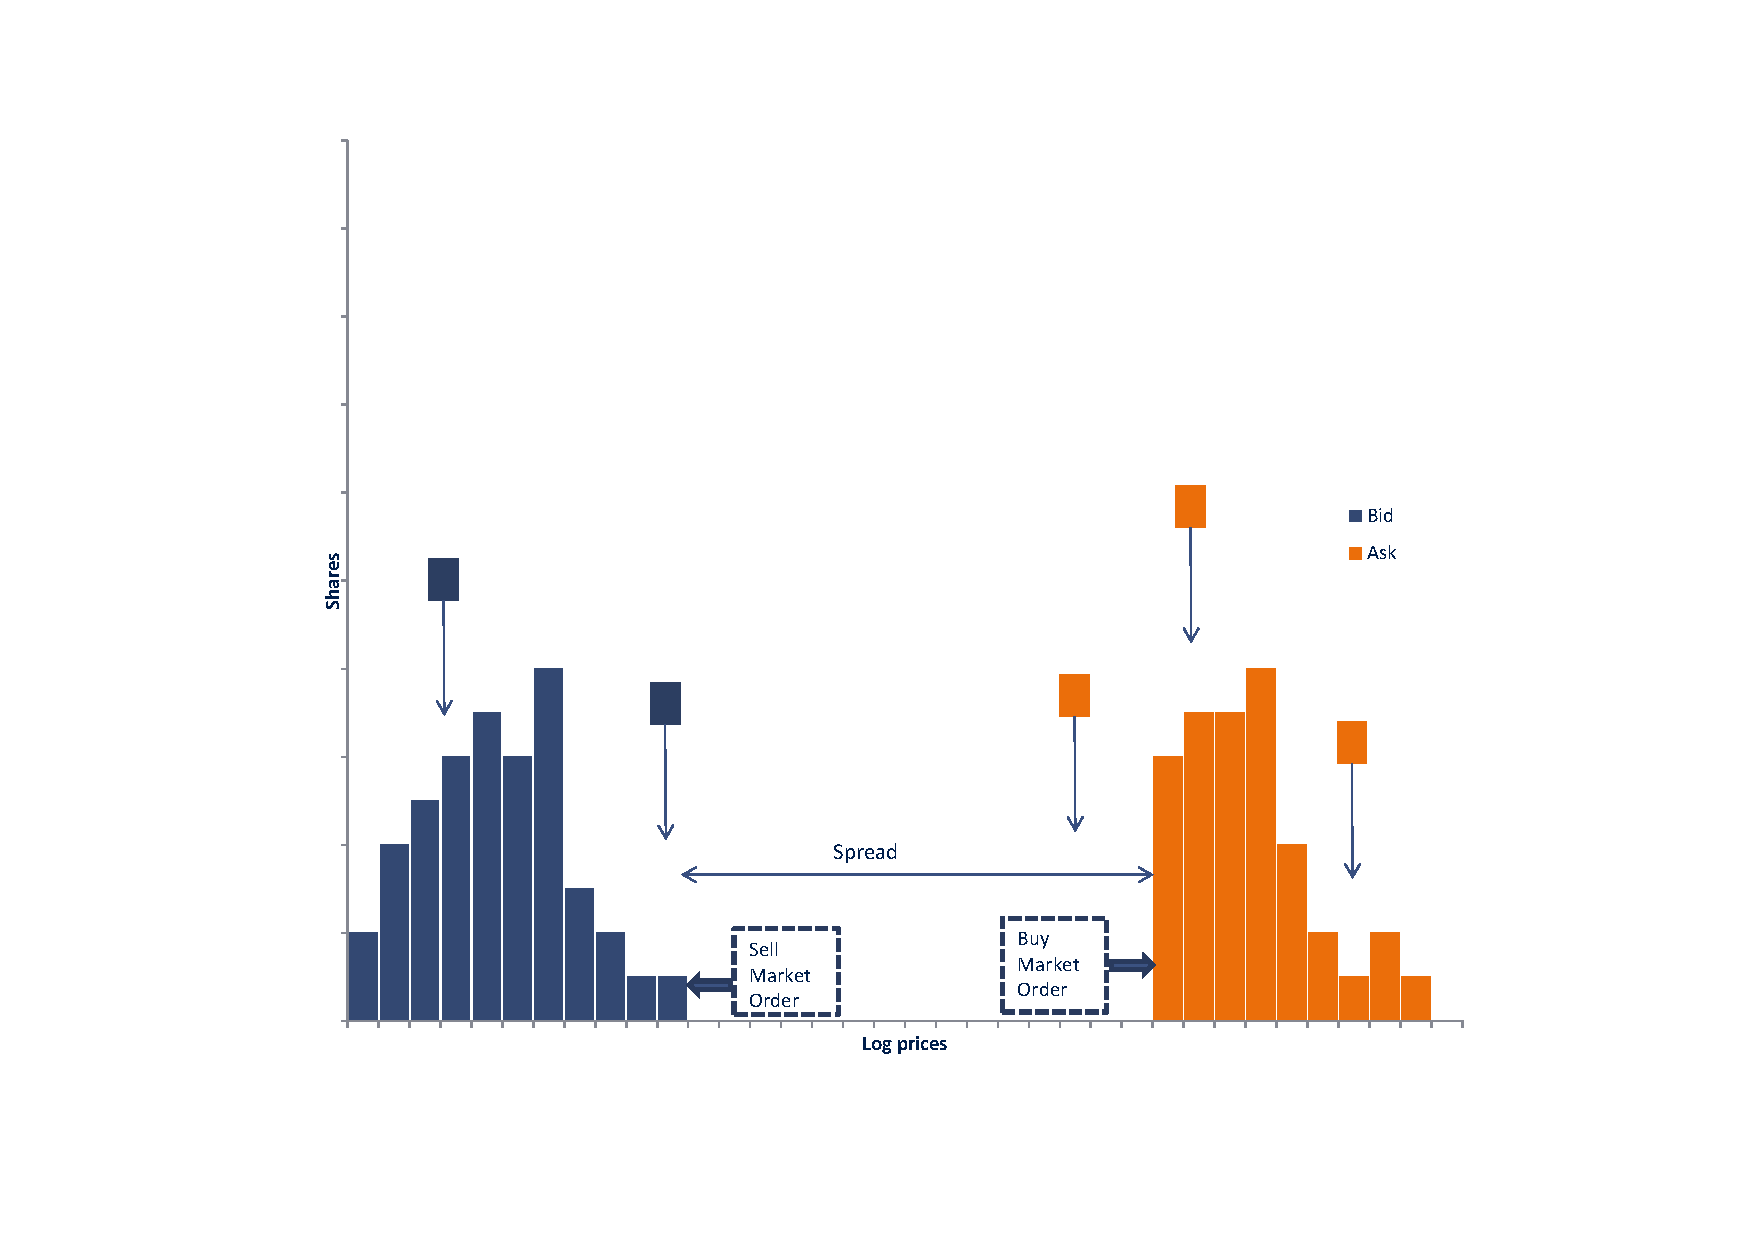
\includegraphics[width=1\textwidth]
		{Continuous_Auction_Model.pdf}
		\caption{Model of a double auction. Limit order are stored in a limit order book. 
		By contrast market orders are executed immediately.}
		\label{exercise_boundary_amaerican_option_fd}
	\end{center}		
\end{figure}

%****************************************************************************************
% Modelling of order flows
% [TODO] I also think that the writing here could be 
% a bit clearer. At the moment, you're providing a general big-picture overview of what 
% happens in the model, but because the clarity dips in a few places, it's hard for 
% the reader to get a clear and detailed understanding of how the model actually works. 
% I'd propose that you think about a short bullet-point list of the things that you want 
% to cover in this material (and that will be understandable to a reader), and then 
% that you re-order the things you're presenting here to support that list.
%****************************************************************************************

\chapter{Modelling the order flow}
\label{chapter:order_flow_model}

%%-----------------------------------------------------------------------------------------
% Introduction
%-----------------------------------------------------------------------------------------

In this chapter we introduce an order flow model first proposed by \citeauthor{Smith:2003:StatisticalModel}~\cite{Smith:2003:StatisticalModel}. In this thesis we will refer to this model as \ac{sfgk}. \ac{sfgk} models the arrivals of orders into at a \ac{lob} using simple stochastic processes. 
The idea by \citeauthor{Smith:2003:StatisticalModel} was to create analytically tractable model while keeping the key features of the continuous double auction that we introduced on Chapter~\ref{chapter:double_auction}. The model can be thought of as a set of a zero-intelligent traders submitting \acp{lo} and \acp{mo} into a \ac{lob}. Zero-intelligent in this context means that there are no learning features that drive the trader's behaviour.
\\
\\
\noindent The chapter is organized as follows: In Sec.~\ref{section:order_flow_model:theory} we will describe the model in more detail. Subsequently, we will describe the algorithm in Sec.~\ref{section:order_flow_model:algorithm} as foundation for the following implementation in Sec.~\ref{section:implementation:order_flow_model}. 

%-----------------------------------------------------------------------------------------
% Theoretical description of the model
%-----------------------------------------------------------------------------------------

\section{Theory}
\label{section:order_flow_model:theory}
% Buy and sell orders are equally likely and hence occur at the same rate. 
% Smith model zero-intelligents tardes by three statistcal poisson prcessed which are correlated only by the LOB. 
Using Poisson processes \citeauthor{Smith:2003:StatisticalModel}~\cite{Smith:2003:StatisticalModel, Daniels:2001:storing} model all orders flowing into the \ac{lob}. Note, as we highlighted in Sec.~\ref{section:poisson:arrival_process} the definition of the Poisson process as in terms of an arrival process, makes it suitable for modelling the times at which events, e.g. the submission of a \ac{lo} or \ac{mo}, arrive at a \ac{lob}. In the following sections, we explain the rates of the different order flows in more detail:
	
\subsection{Market order events}

\acp{mo} arrive into the \ac{lob} in chunks of $\sigma$ shares at a rate of $\mu$ shares per unit of time. Sell and buy \acp{mo} are equally likely. Market orders are executed immediately by being matched to the corresponding limit order in the \ac{lob}. Hence a buy \ac{mo} removes an offer at the price $a(t)$. If thereby, the last offer was removed, $a(t)$ moves up to the next occupied best price level on  the sell side. Analogously, a sell \ac{mo} removes an offer at $b(t)$. If the last offer was removed, $b(t)$ moves down to the next occupied best price level on  the buy side.

\subsection{Limit order events} 

\acp{lo} arrive into the \ac{lob} in chunks of $\sigma$ shares and with a limit price in chunks of $\pi$ at a rate of $\alpha$ shares per unit of time and per unit of price. The probability being a sell or buy \ac{lo} is equal. The limit price $p$ of an order is drawn in quanta of $\pi$ from a uniform distribution on the interval $(b(t), \infty)$ for sell orders and on $(-\infty, a(t))$ for buy orders.

\subsection{Cancellation events} 

\acp{lo} placed in the \ac{lob} expire randomly with a rate $\delta$ per unit time.
\\
\\
\noindent All parameters are summarized in Table~\ref{table:model_parameter}. The order rates $\alpha$, $\mu$ and $\delta$ can be understood as parameters characterizing the trading behaviour of a set of zero-intelligent agents. By contrast, the tick size $\pi$ and $\sigma$ accounts for the fact, that in a real-world setting stocks are traded in discrete price and size quanta. 
%
%-----------------------------------------------------------------------------------------
% Table: Model parameter
%-----------------------------------------------------------------------------------------

\begin{table}    
    \begin{tabular*}{\textwidth}{l @{\extracolsep{\fill}} ll}
    	\hline    	
		{\bf Parameter}	& {\bf Description}				& {\bf Unit} \\
    	\hline
		$\alpha$	& Average \ac{lo} rate 				& \# of shares/price$\cdot$time \\	
		$\mu$		& Average \ac{mo} rate 				& \# of shares/time \\	
		$\delta$	& Average \ac{lo} cancellation rate	& 1 / price\\	
		$\sigma$	& Size of an order					& \# of shares\\	
		$\pi$		& Tick size	 						& price\\	
		\hline
    \end{tabular*}
    \caption{Overview of the parameters characterizing the \ac{sfgk}. While $\alpha$, $\mu$ and $\delta$ can be interpreted as the parameters that drive the zero-intelligent agents, $\sigma$ and $\pi$ are discreteness parameters that reflect the fact that trading assets can only be traded in discrete price and size quanta.}
    \label{table:model_parameter}
\end{table}

%-----------------------------------------------------------------------------------------
% Slight modification of the model
%-----------------------------------------------------------------------------------------

\section{Practical simplification}
\label{section:order_flow_finite_interval}

The placement of \acp{lo} on an infinite interval makes the model analytically more tractable 
as it ensures that there is always an infinite number of \acp{lo} stored in the \ac{lob}, hence, keep the \ac{lob} at all times in well-defined states ($a(t)$ and $b(t)$ are always defined) ~\cite{Smith:2003:StatisticalModel}. From a technical angle, however, drawing prices from an infinite interval renders any implementation infeasible. Therefore, we will slightly modify the model for practical reasons, by introducing a sufficiently large cap $L$ for the price interval: The price of buy \acp{lo} is drawn from a uniform distribution on the interval $(a(t)-L, a(t)]$. Similarly, the price of sell \acp{lo} is drawn from a uniform distribution on the interval $(b(t), b(t)+L]$.

%-----------------------------------------------------------------------------------------
% Algorithm for model, Check p 34 lectture notes, M. Gould describes a general model 
%-----------------------------------------------------------------------------------------

\section{Algorithm}
\label{section:order_flow_model:algorithm}

In this section we formulate a simulation algorithm of the \ac{sfgk} that we have introduced in Sec.~\ref{section:order_flow_model:theory}. To this end, we will first describe the data structure to store the state of the the \ac{lob} introduced in Sec.~\ref{section:lob}. Second, we will describe events and how they impact the \ac{lob}, and, finally, we focus our attention on the mathematical description of the order flow.

%----------------------------------------------------------------------------------------
%
% Structure of the LOB
%
%-----------------------------------------------------------------------------------------

\subsection{Limit order book}
We model the \ac{lob} solely in terms of its depth profile (see Sec.~\ref{section:lob}) as we are only interest in the price evolution. To this end, we first define the discrete set of prices by,
% 
\begin{eqnarray}
	P=\lbrace p_1, p_2, p_3,..., p_n\rbrace,
\end{eqnarray}
%
therein, the prices are equidistant with size $\pi$.
%
The depth profile at any given time $t$ of the \ac{lob} is modelled by the vector, 
%
\begin{eqnarray}
	\mathbf{Y}(t)=\left(Y_{p_1}(t), Y_{p_2}(t), Y_{p_3}(t), ..., Y_{p_n}(t)\right),
\end{eqnarray} 
%
therein, $Y_p(t)$ denotes the depth available at price $p$ at time $t$. Note, that sell orders have positive and buy order negative depth (see convention in Sec.~\ref{section:lob}). Next, we define the bid by, 
%
\begin{eqnarray}
	b(t) = \max\lbrace p\in P|Y_p(t) < 0 \rbrace
	\label{algorithm:bid_price}
\end{eqnarray}
%
and ask price at time $t$ by,
%
\begin{eqnarray}
	a(t)=\min\lbrace p\in P| Y_p(t) > 0\rbrace.
	\label{algorithm:ask_price}
\end{eqnarray} 
%
In case the buy side of the \ac{lob} is empty, in other words the maximum in Eq.~\ref{algorithm:bid_price} cannot be defined, we $b(t)=\min P$. Similarly, if the sell side is empty and therefore the minimum in Eq.~\ref{algorithm:ask_price} is undefined,  we set $a(t)=\max P$.

%----------------------------------------------------------------------------------------
%
% Order Events
%
%-----------------------------------------------------------------------------------------

\subsection{Order events}
\label{section:algo:order_events}

After having defined the structure of the \ac{lob}, we define the events that arrive at time $t$ at the \ac{lob}, thereby changing its depth profile $\mathbf{Y}$:
%
\begin{itemize}
	\item $L_B$: Buy limit order at price $p$: $\mathbf{Y}(t^+)=\mathbf{Y}(t^-)-\mathbf{e}_p$, 
	where the price $p$ is drawn from a uniform distribution on the interval $[a(t^-)-L,a(t^-)]$ 
	in units of $\pi$.
	
	\item $L_S$: Sell limit order at price $p$: $\mathbf{Y}(t^+)=\mathbf{Y}(t^-)+\mathbf{e}_p$, 
	where the price $p$ is drawn from a uniform distribution on the interval $[b(t^-),b(t^-)+L]$ 
	in units of $\pi$.
	\item $M_B$: Buy market order causes: $\mathbf{Y}(t^+)=\mathbf{Y}(t^-)-\mathbf{e}_{a(t^-)}$
	
	\item $M_B$: Sell market order at price causes: $\mathbf{Y}(t^+)=\mathbf{Y}(t^-)+\mathbf{e}_{b(t^-)}$
	
	\item $C_B$: A cancellation of an active buy order at price $p$: 
	$\mathbf{Y}(t^+)=\mathbf{Y}(t^-)+\mathbf{e}_p$,
	where the price $p$ is drawn from a uniform distribution on the interval $[b(t^-)-L,b(t^-)]$ 
	in units of $\pi$. 

	\item $C_S$:  A cancellation of an active sell order at price $p$ causes : 
	$\mathbf{Y}(t^+)=\mathbf{Y}(t^-)-\mathbf{e}_p$,
	where the price $p$ is drawn from a uniform distribution on the interval $[a(t^-),a(t^-)+L]$ 
	in units of $\pi$.  	
\end{itemize}
%
therein, $\mathbf{Y}(t^+)=\lim _{t\to t^+}\mathbf{Y}(t)$ is depth profile at an infinitesimal small step after the event occurred. Analogously, $\mathbf{Y}(t^-)=\lim _{t\to t^-}\mathbf{Y}(t)$ is depth profile at an infinitesimal small before the event occurred. $\mathbf{e}_p$ denotes the unit vector, being $0$ at all position except at $p$. $L$ is the finite simulation interval size (see Sec.~\ref{section:order_flow_finite_interval}). Moreover, $a(t^-)=\lim _{t\to t^-}a(t)$ and $b(t^-)=\lim _{t\to t^-}b(t)$, being the ask and the bid price prior to the event, respectively.

%----------------------------------------------------------------------------------------
%
% Order flow
%
%-----------------------------------------------------------------------------------------

\subsection{Order Flow}
\label{section:algo:simulation}

In the following we describe all simulation steps of the \ac{sfgk}, beginning with initialisation and followed by the incremental time steps that are repeated until the maximal  simulation period is reached.

%---------------------------------------------------------------------------------------
% Step 0: Simulation process 
%---------------------------------------------------------------------------------------

\paragraph{Step 0} The simulation is initialized by,

\begin{eqnarray}
		t_0 &=& 0
		\\\nonumber
		\mathbf{Y(0)} &=& \mathbf{Y}_0
\end{eqnarray}

%---------------------------------------------------------------------------------------
% Step i: Simulation process 
%---------------------------------------------------------------------------------------

\paragraph{Step i} The $i^\textrm{th}$ step of the simulation consists of the following procedure, 

\begin{itemize}

	\item Set the rates for the events described in Sec.~\ref{section:algo:order_events} taking into 
	account that sell and buy are equally likely, 
	\begin{eqnarray}
		\lambda_{L_B} &=& \alpha/2\,(s(t)+L)
		\\\nonumber	
		\lambda_{L_S} &=& \alpha/2\,(s(t)+L)
		\\\nonumber	
		\lambda_{M_B} &=& \mu/2
		\\\nonumber	
		\lambda_{M_S} &=& \mu/2
		\\\nonumber	
		\lambda_{C_B} &=& \delta/2\,n_\textrm{b}(t)
		\\\nonumber	
		\lambda_{C_S} &=& \delta/2\,n_\textrm{a}(t),
	\end{eqnarray}
	therein, $n_a(t)$ is the number of active sell \acp{lo}, 
	with prices within the interval $[a(t), a(t)+L]$ at time $t$. Similarly, $n_b(t)$ 
	is the number of active buy \acp{lo} with prices within the interval $[b(t)-L, b(t)]$ at time $t$. 
	Moreover, $s(t)$ is the spread at time $t$.
	
	\item Using the merging property of the Poisson processes as described in 
	Theorem~\ref{theorem:poisson_merging}, we set the total event rate,
	\begin{eqnarray}
		\lambda = 
		\lambda_{L_B} + \lambda_{L_S} + 
		\lambda_{M_B} + \lambda_{M_S} + 
		\lambda_{C_B} + \lambda_{C_S}.
	\end{eqnarray}
	
	\item Using the definition ~\ref{section:poisson:arrival_process}, we select a random 
	interrarival time $X_i$ by 
	\begin{eqnarray}
		X_i \sim f_{X_i}(x) = \lambda\,e^{-\lambda\,x}
	\end{eqnarray}

	\item Assign each event to its probability by, 
	\begin{eqnarray}
		\mathbb{P}(L_B) &=& \frac{\lambda_{L_B}}{\lambda}
		\label{equation:algo:probabilities_events}
		\\\nonumber		
		\mathbb{P}(L_S) &=& \frac{\lambda_{L_S}}{\lambda}
		\\\nonumber
		\mathbb{P}(C_B) &=& \frac{\lambda_{C_B}}{\lambda}
		\\\nonumber
		\mathbb{P}(C_S) &=& \frac{\lambda_{C_S}}{\lambda}
		\\\nonumber
		\mathbb{P}(M_B) &=& \frac{\lambda_{M_B}}{\lambda}	
		\\\nonumber
		\mathbb{P}(M_S) &=& \frac{\lambda_{M_S}}{\lambda}.	
	\end{eqnarray}
	Draw an event $E$ from $\lbrace L_B,L_S,C_B,C_S,M_B,M_S\rbrace$ 
	with the probabilities as defined in Eq.~\ref{equation:algo:probabilities_events}. 
	
	\item Execute the event $E$ by changing the depth profile $Y(t_{i-1})$ according to 
	Sec.~\ref{section:algo:order_events} and save the result in $Y(t_{i})$.
	
	\item Increase the time $t_{i} = X_i + t_{i-1}$
\end{itemize}

%***********************************************************************************
%
% Methods
%
%***********************************************************************************

\chapter{Materials \& Methods}
\label{chapter:material_methods}

%------------------------------------------------------------------------------------
% Short introduction
%------------------------------------------------------------------------------------

In this chapter we review the materials and methods central within the framework of this thesis.
%
%-----------------------------------------------------------------------------------------
% Structure of the chapter 
%-----------------------------------------------------------------------------------------
%
\noindent This chapter as structured as follows: 
%
%-----------------------------------------------------------------------------------------
% Data
%-----------------------------------------------------------------------------------------
%
We start this chapter with Sec.~\ref{section:methods:data} where we describe the structure of the trading data and present its key features. 
%
%-----------------------------------------------------------------------------------------
% Data  treatment
%-----------------------------------------------------------------------------------------
%
In Sec.~\ref{section:methods:data_treatment} we describe how the data is pre-processed for the simulation.
%
%-----------------------------------------------------------------------------------------
% Section: Calibration
%-----------------------------------------------------------------------------------------
%
In Sec.~\ref{section:methods:calibration} we then elaborate on how the order flow rates and discretisation parameters of the \ac{sfgk} (see Chapter~\ref{chapter:order_flow_model}) can be determined from the trading data. 
%
%-----------------------------------------------------------------------------------------
% Section: Simulation
%-----------------------------------------------------------------------------------------
%
Sec.~\ref{section:simulation} gives an overview of the simulation. 
%
%-----------------------------------------------------------------------------------------
% Section: Analysis
%-----------------------------------------------------------------------------------------
%
The chapter concludes with Sec.~\ref{section:analysis} where we discuss how that data obtained from the simulation was analysed to finally produce the model-implied realized volatility.
%
%------------------------------------------------------------------------------------
% Data 
%------------------------------------------------------------------------------------

\section{Data}
\label{section:methods:data}
In order to get real-world data for calibration of the order flow model and for testing the predictably of the estimated realized volatility we use trading data sets from the \ac{lobster} project. The \ac{lobster} projected, affiliated with the Humboldt University and the University of Vienna, serves the academic community  with reconstructed limit order book data for the entire universe of \ac{nasdaq} traded stocks. For more information about the project please refer to their website \href{https://lobsterdata.com/}{https://lobsterdata.com/}. 
\\
% Shortly described the structure of of the LOBSTER data
For each stock and trading day the \ac{lobster} data sets consists of two separate files, described in the following paragraphs: 

\paragraph{Event file} The Event file consists of a list of time-stamped events that caused an update of the state of the \ac{lob}. In the following we list all events types that can occur, 
\begin{itemize}
	\item Submission of a new limit order
	\item Cancellation (partial deletion of a limit order)
	\item Deletion (total deletion of a limit order)
	\item Execution of a visible limit order
	\item Execution of a hidden limit order
	\item Cross trade, e.g. auction trade
	\item Trading halt indicator
\end{itemize}

\paragraph{State file} The state file, which is linked by means of a time-stamp to the first one, consists of the states of the \ac{lob}. Here the state of the \ac{lob} is the total volume of outstanding limit orders on the bid and ask side up to a the first $n$ best price levels. 
\\
\\
\noindent A detailed description of the data structure can be found on the \ac{lobster} \href{https://lobsterdata.com/info/DataStructure.php}{website}. 
\\
In this thesis we focus on $3$ sets of data for the stocks \ac{amzn}, \ac{tsla} and \ac{nflx} for trading days ranging from $4^\textrm{th}$ to $29^{\textrm{th}}$  January $2016$ and fixed price level $n=10$. 

Table~\ref{table:statistics:trading_data} depicts the average rates for different event types for the trading day $4^\textrm{th}$ January $2016$ for the tickers \ac{amzn}, \ac{nflx} and \ac{tsla}. 
% TODO: Cite that the majority of LOs are either cancelled or deleted from the limit order book
For \ac{amzn} we observe a very high buy pressure as the submission rate for \ac{lo} on the buy side is larger than the sell side. By contract, \ac{nflx} and \ac{tsla} exhibit a higher selling pressure. It is noticeable that for all stocks that the majority of outstanding \acp{lo} are not executed by matching with a corresponding \ac{mo} but either partly or totally deleted. This is behaviour particularly stresses the importance of accurately modelling the cancellation rate of \acp{lo} in a order-flow model.
%
% Table: Average rate (order events / sec) for different order types 
% for whole trading data (in + out-of-sample) 
% TODO: Vertical spacing in tabular environment
% Source: results\{stock}\{tardingDay}\statistics_all.json
\begin{table}    
    \begin{tabular*}{\textwidth}{l @{\extracolsep{\fill}} ccc}
    	\hline    	
		{\bf Stock} 				&{\bf\ac{amzn}} 		&{\bf \ac{nflx}} 		&{\bf \ac{tsla}}
		\vspace{1mm} \\
    	\hline
		Submission (buy)			& $3.53$ 				& $5.21$ 				& $1.50$ \\
		Submission (sell)			& $1.94$ 				& $6.19$ 				& $2.04$ \\
	  	Cancelled (buy)  			& $5.98\cdot 10^{-4}$ 	& $4.60\cdot 10^{-2}$	& $8.97\cdot 10^{-4}$ \\
  		Cancelled (sell)			& $4.44\cdot 10^{-4}$ 	& $1.79\cdot 10^{-2}$	& $1.75\cdot 10^{-3}$ \\
	  	Deleted (buy)				& $3.28$ 				& $4.76$ 				& $1.30$ \\
  		Deleted (sell)				& $1.72$ 				& $5.70$ 				& $1.80$ \\
		Executed visible (buy)		& $0.44$ 				& $0.53$	 			& $0.31$ \\
  		Executed visible (sell)		& $0.36$ 				& $0.54$	 			& $0.26$ \\
		Executed hidden (buy)		& $0.50$ 				& $0.46$	 			& $0.28$ \\
  		Executed hidden (sell)		& $0$  					& $0$		 			& $0$ \\
	    \hline
    \end{tabular*}
    \caption{Event rates in units of number of events per second for the 
    stocks \ac{amzn}, \ac{nflx} and \ac{tsla} for the trading day $4^\textrm{th}$ January $2016$. }
    \label{table:statistics:trading_data}
\end{table}

%------------------------------------------------------------------------------------
% Data Treatment
%------------------------------------------------------------------------------------

\section{Data Treatment}
\label{section:methods:data_treatment}

%------------------------------------------------------------------------------------
% Table with in-sample and out of sample data 
%------------------------------------------------------------------------------------

\begin{table}[ht]
    \begin{tabular*}{\textwidth}{l|l| @{\extracolsep{\fill}} cc|cc}
    	\hline 
    				&   			 	 & \multicolumn{2}{c|}{\bf In-sample} & \multicolumn{2}{c}{\bf Out-of-sample} \\
		\hline
		{\bf Stock} & {\bf Trading date} & {\it Start} 	& {\it End}      & {\it Start} 	& {\it End} \\
    	\hline
    			  & $2016-01-04$ 		 & 			&  					  & 		& 		  \\
    	\ac{amzn} & $2016-01-15$ 		 & $09:30$	& $13:13$ 			  & $13:13$ & $16:00$ \\
    			  & $2016-01-29$ 		 & 			&    	 			  & 		& 		  \\
    	\hline
    			  & $2016-01-04$ 		 & 			& 		 			  & 		& 		  \\
    	\ac{nflx} & $2016-01-15$ 		 & $09:30$	& $13:13$ 			  & $13:13$ & $16:00$ \\
    			  & $2016-01-29$ 		 & 			& 		 			  & 		& 		  \\
    	\hline
    			  & $2016-01-04$ 		 & 			& 		 			  & 		& 		  \\
    	\ac{tsla} & $2016-01-15$ 		 & $09:30$	& $13:13$ 			  & $13:13$ & $16:00$ \\
    			  & $2016-01-29$ 		 &			& 		 			  & 		& 		  \\
    	\hline

    \end{tabular*}
    \caption{For each stock and trading date the data sets from the \ac{lobster} 
    was split into an in-sample and out-of sample data set.}
    \label{table:in_sample_out_of_sample}
\end{table}

\noindent In order to gauge the \ac{sfgk} forecasting performance, we split the trading data, which cover the regular market hours from $09:00$ till $16:00$, into two data sets: 

\begin{itemize}
	\item In the {\it in-sample data} that cover the trading time from $09:30$ till  $13:13$. 
	This subset of trading data will be use to calibrate the \ac{sfgk}, 
	as described in Sec~\ref{section:methods:calibration}.
	
	\item and the {\it out-of-sample data}. We will later used this subset of the trading data to empirically determine the realized volatility.
\end{itemize}

\noindent Note that the out-of-sample trading data covers a trading duration of $10^4s$. This will be later for the simulation period of the \ac{sfgk}. Table~\ref{table:in_sample_out_of_sample} summarizes the splitting of the trading data for future reference.

%------------------------------------------------------------------------------------
% Data Treatment
%------------------------------------------------------------------------------------

\section{Calibration}
\label{section:methods:calibration}

%-----------------------------------------------------------------------------------------------
% Introduction
%-----------------------------------------------------------------------------------------------

Using the the in-sample trading data (see Sec.~\ref{section:methods:data_treatment}), we determine the parameters of the \ac{sfgk} (see Table~\ref{table:model_parameter}) using the steps that are presented the following sections.

%-----------------------------------------------------------------------------------------------
% Simulation window
%-----------------------------------------------------------------------------------------------

\subsection{Calibration window}

Before starting with calibrating the parameters of the \ac{sfgk}, we determine a small calibration window near the spread. We define this window, denoted by $[q_l, q_u]$, by the $1$\% and $80$\%  quantiles of the time-averaged limit order depth distribution Eq~\ref{equation:time_averaged_depth_profile}. Here, we make the compromise between including as much data as possible for calibrating and excluding limit orders that are unlikely to be executed. 
\\
\\
\noindent The reasoning behind this is, when calibrating the limit order and cancellation rates (see Sec.~\ref{section:methods:calibrate_alpha} and \ref{section:methods:calibrate_delta}), a problem occurs due to the simplifying assumption of the \ac{sfgk} of a uniform distribution of prices for limit order placement and a uniform cancellation rate (see Chapter~\ref{chapter:order_flow_model}). In the real data, limit order placement and cancellation are concentrated near the best prices~\cite{Bouchaud:2002:statistical}. This situation is visible in Fig.~\ref{figure:methods:simulation_windows}, where we observe that the depth of limit orders far away from the spread decays as a power law function of the distance from the best prices. Within a narrow window we can assume that the uniform distribution of prices for limit order placement and a uniform cancellation rate is justified. 

%-----------------------------------------------------------------------------------------------
% Figure: Average depth profile for AMZN, 4th Januay 2016.
%-----------------------------------------------------------------------------------------------
   
\begin{figure}[htp]	
	\centering
    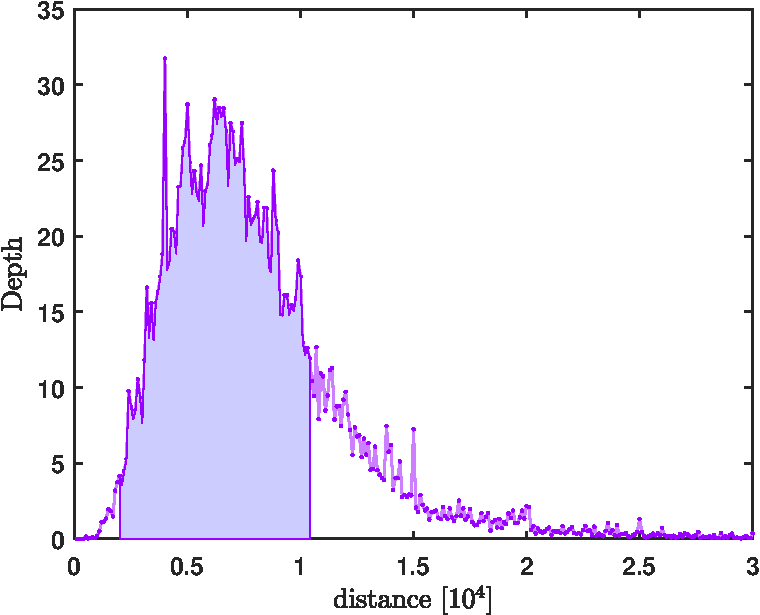
\includegraphics[width=\textwidth]{./AverageDepthProfile/AMZN/average_depth_profile.pdf}
	\caption{Average depth profile of \ac{amzn} for the trading day $4^\textrm{th}$ January $2016$. 
	The solid blue area below the graph is bounded by the $1$\% and $80$\% quantiles of 
	the distribution. Most of the limit orders are placed near the spread. The depth of limit orders far away from the spread decays as a power law function of the distance from the best prices.}
	\label{figure:methods:simulation_windows}
\end{figure}

%-----------------------------------------------------------------------------------------------
% Tick size
%-----------------------------------------------------------------------------------------------

\subsection{Tick size} 

As the difference between two price levels in the state file of the in-sample data is not necessarily the minimum tick size, we heuristically measure the parameter $\pi$ by computing the greatest common divisor of all non-zero positive price differences.

%-----------------------------------------------------------------------------------------------
% Characteristic size
%-----------------------------------------------------------------------------------------------

\subsection{Characteristic order size} 

We obtain the characteristic size $\sigma$ by taking the mean of all sizes of all \acp{lo} and \acp{mo} submitted to the \ac{lob}. 

%-----------------------------------------------------------------------------------------------
% Market order rate 
%-----------------------------------------------------------------------------------------------

\subsection{Market order rate} 

The measurement of the market order rate $\mu$ is straightforward: We compute the sum of the size of all \acp{mo}, denoted by $V_\textrm{MO}$,  and finally obtain $\mu$ by,

\begin{eqnarray}
	\mu = \frac{V_\textrm{MO}}{\sigma\cdot T},
\end{eqnarray}

\noindent therein T being the total trading duration of the in-sample-data.
%-----------------------------------------------------------------------------------------------
% Limit order rate
%-----------------------------------------------------------------------------------------------

\subsection{Limit order rate} 
\label{section:methods:calibrate_alpha}

In order to determine the limit order rate $\alpha$, we compute the total size $V_\textrm{LO}$ of all limit orders whose distance with respect to the best opposite quote is bounded by the lower and the upper quantile, denoted by $q_l$ and $q_u$, respectively. Finally, $\alpha$ is obtain by, 

\begin{eqnarray}	
	\alpha = \frac{V_\textrm{LO}}
	{\sigma\cdot (q_u - q_l)/\pi\cdot T}.
\end{eqnarray}

%-----------------------------------------------------------------------------------------------
% Cancellation rate 
%-----------------------------------------------------------------------------------------------

\subsection{Cancellation rate}
\label{section:methods:calibrate_delta}
The determination of the cancellation rate $\delta$ from the in-sample data required several steps. First,
we compute the time-averaged total size of active limit order in the \ac{lob} within the distance window $[q_l, q_u]$ by,

\begin{eqnarray}
	N_\textrm{LO} &=& \int_{q_l}^{q_u} 
	n\left(s, [T_\textrm{start}, T_\textrm{end}]\right)\,\dd s,
\end{eqnarray}
%
therein, $n$ is the time-averaged depth profile Eq. \ref{equation:time_averaged_depth_profile} over the whole trading time, denoted by the interval $[T_\textrm{start}, T_\textrm{end}]$. Second, we compute the total size of cancellations of limit orders in the same window $[q_l, q_u]$, denoted by $V_\textrm{CO}$. Finally, we obtain $delta$ by, 

\begin{eqnarray}
	\delta &=& \frac{V_\textrm{CO}}{N_\textrm{LO}\cdot\left\lvert T_\textrm{in}\right\rvert}.
\end{eqnarray}


%------------------------------------------------------------------------------------
% Simulation
%------------------------------------------------------------------------------------

\section{Simulation}
\label{section:simulation}
After having calibrated the \ac{sfgk} to the in-sample data as explained in detail in Sec.~\ref{section:methods:calibration}. We run a set of $k= 1,...,10$ simulations of length $10^4$ seconds of the model employing the algorithm described in Sec.~ \ref{section:algo:simulation}.
Thereby, we set the simulation interval length $L=4*s(0)$, there $s(0)$ denotes the initial spread. Furthermore, we set the initial depth profile $\mathbf{Y}_0$ of the \ac{lob} to be the depth profile in the last time slice of the state file in the in-sample data.

%------------------------------------------------------------------------------------
% Analysis of simulation results
%------------------------------------------------------------------------------------

\section{Analysis}
\label{section:analysis}

As result for each simulation, we get a set of depth profiles,
%
\begin{eqnarray}
	\left\lbrace \mathbf{Y}^{(k)}(t_{i_k}), i_k = 0, ..., N_k \right\rbrace	
\end{eqnarray}
%
therein, $k$ denotes the path, $N_k$ is the number of order events that changed the state of the depth profile (see Chapter~\ref{chapter:order_flow_model}) and $t_{i_k}$ is the arrival time of an order event. Note the the interarrival time between two evens is $\tau_{i_k}=t_{i_k}-t_{i_k-1}$ (see Chapter ~\ref{chapter:poisson_process}).

%------------------------------------------------------------------------------------
% Simulated Proce
%------------------------------------------------------------------------------------

\subsection{Price}
\label{section:methods:price}

Using Eq.~\ref{algorithm:bid_price} and Eq.~\ref{algorithm:ask_price}, we determine the bid and ask price. Averaging the bid and ask price for each time step, we finally get the model-implied price, 
%
\begin{eqnarray}
	\left\lbrace p^{(k)}(t_{i_k})=[a^{(k)}(t_{i_k})+b^{(k)}(t_{i_k})]/2, i_k = 0, ..., N_k\right\rbrace 
	\label{equation:analysis:price_time_series}
\end{eqnarray}
%
therein, $a^{(k)}(t_{i_k})$ and $b^{(k)}(t_{i_k})$, is the bid price and the ask price, respectively.

%------------------------------------------------------------------------------------
% Model-Implied RV
%------------------------------------------------------------------------------------

\subsection{Model-Implied Realized volatility}

The model-implied realized volatility is computed using Eq.~\ref{equation:realized_volatility_estimator} from the price time series in Eq.~\ref{equation:analysis:price_time_series} by first re-sampling the series to a regularly spaced time grid of size $\delta T = 10\,$ms using linear interpolation.

%------------------------------------------------------------------------------------
% Empirical RV
%------------------------------------------------------------------------------------

\subsection{Empirical Realized volatility}


\label{section:methods:empirical_realized_volatility}

The empirical realized volatility is directly estimated from the out-of-sample data by applying Eq.~\ref{equation:realized_volatility_estimator}. To this end we extract the price process from the state file of the trading data by computing the mid price Eq.~\ref{equation:mid_price} from the best bid and ask prices.

%***********************************************************************************
%
% Results
%
%***********************************************************************************

\chapter{Results}
\label{chapter:results}

%-----------------------------------------------------------------------------------------
% Introduction
%----------------------------------------------------------------------------------------

In this section we focus on the results of this thesis by discussing the prediction performance of the \ac{sfgk} with respect to the realized volatility for three stocks, namely, \ac{tsla}, \ac{amzn} and \ac{nflx} for the trading days $4^\textrm{th}$, $15^\textrm{th}$ and $29^\textrm{th}$ January $2016$. To test the predictability, we have split the trading data into in- and out-of-sample subsets. Using the in-sample data we calibrated the \ac{sfgk} and produced predictions for the realized volatility, also termed {\it model-implied realized volatilities}, that we compare with the empirical realized volatility observed in the out-of sample data (see Chapter~\ref{chapter:material_methods}).
\\
\\
\noindent The chapter is structured as follows: We start with discussing the calibration results Sec.~\ref{section:result:calibration}. Then we have a close look at the model-implied price trajectories and compare the predicted and empirical log-return distributions in  Sec.~\ref{section:result:simulation}. In the subsequent Sec.~\ref{section:result:realizedvol} we discuss in detail the volatility signature plots produced by the \ac{sfgk} and finally investigate the forecasting performance of the realized volatility extracted from those signature plots. 

%-----------------------------------------------------------------------------------------
% Calibration
%----------------------------------------------------------------------------------------

\section{Calibration}
\label{section:result:calibration}

%-----------------------------------------------------------------------------------------
% Introduction 
%----------------------------------------------------------------------------------------

In this section we present the calibration results be starting with the calibration window and then present the calibrated parameters of the \ac{sfgk}.

%-----------------------------------------------------------------------------------------
% Calibration window 
%----------------------------------------------------------------------------------------

\subsection{Calibration window}

Before calibrating the parameters of the \ac{sfgk} to the in-sample data, we determine the calibration window by computing the $1$\% and $80$\% quantiles, denoted by $q_l$ and $q_u$, respectively, of the average depth profile. The results for quantiles are shown in the third and fourth column of Table~\ref{table:calibrated_model_parameters}. Fig. \ref{figure:averaged_depth_profile} depicts the calibration window illustrated by a blue solid area below the graph of the the average depth profile of \ac{amzn}, \ac{nflx} and \ac{tsla} for the trading day $4^\textrm{th}$ January $2016$. The depth profile reveals that most limit orders are placed closed to the spread. Moving away from the spread, we can observe that depth of limit orders decays as a power law function of the distance from the best prices. This corroborates our decision to calibrate in a narrow window around the spread as most trading activity will happen there. 

\begin{figure}[htp]	
	
	\centering
	%--------------------------------------------------------------------------------------
	% Average depth profile: Amazon
	%--------------------------------------------------------------------------------------	
	\begin{subfigure}[b]{0.5\textwidth}
    	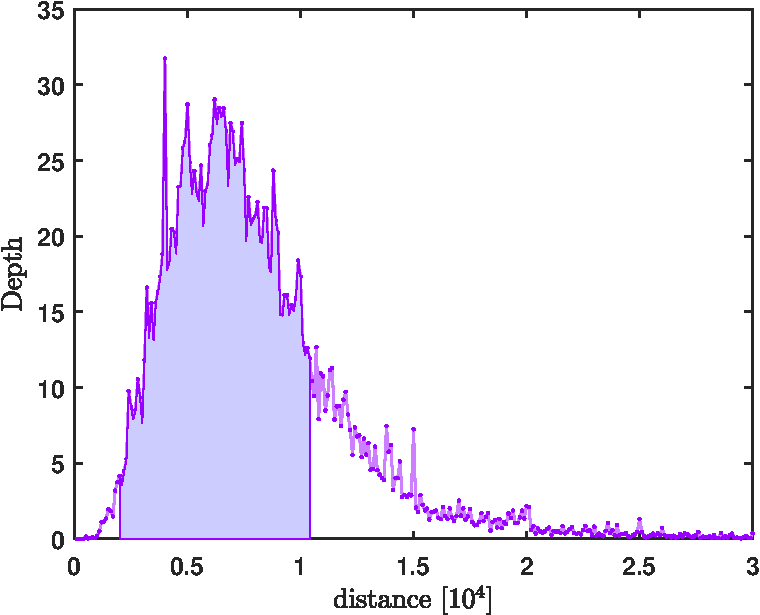
\includegraphics[width=\textwidth]{./AverageDepthProfile/AMZN/average_depth_profile.pdf}
		\caption{\ac{amzn}}
        \label{figure:average_depth:amzn}
	\end{subfigure}
	
	%--------------------------------------------------------------------------------------
	% Average depth profile Netflix	
	%--------------------------------------------------------------------------------------
	\begin{subfigure}[b]{0.5\textwidth}
    	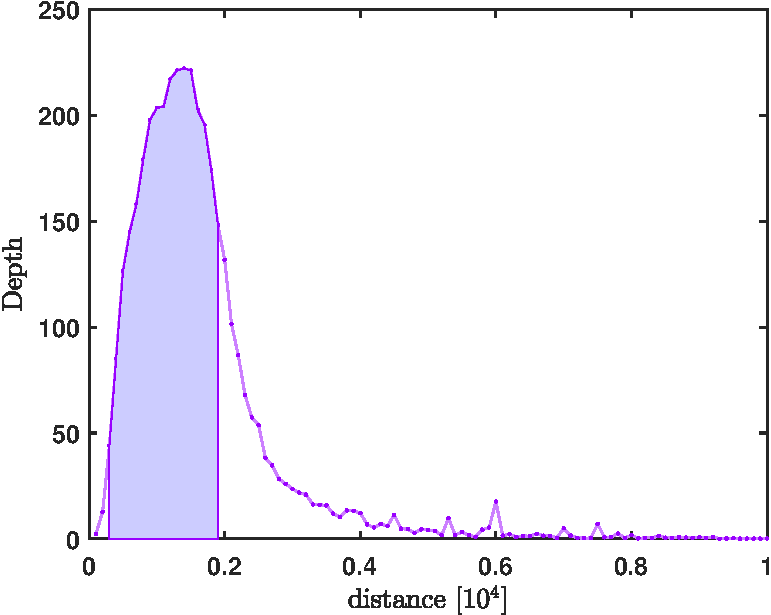
\includegraphics[width=\textwidth]{./AverageDepthProfile/NFLX/average_depth_profile.pdf}
		\caption{\ac{nflx}}
        \label{figure:average_depth:nflx}
	\end{subfigure}
	
	%--------------------------------------------------------------------------------------	
	% Average depth profile Tesla
	%--------------------------------------------------------------------------------------
	\begin{subfigure}[b]{0.5\textwidth}
    	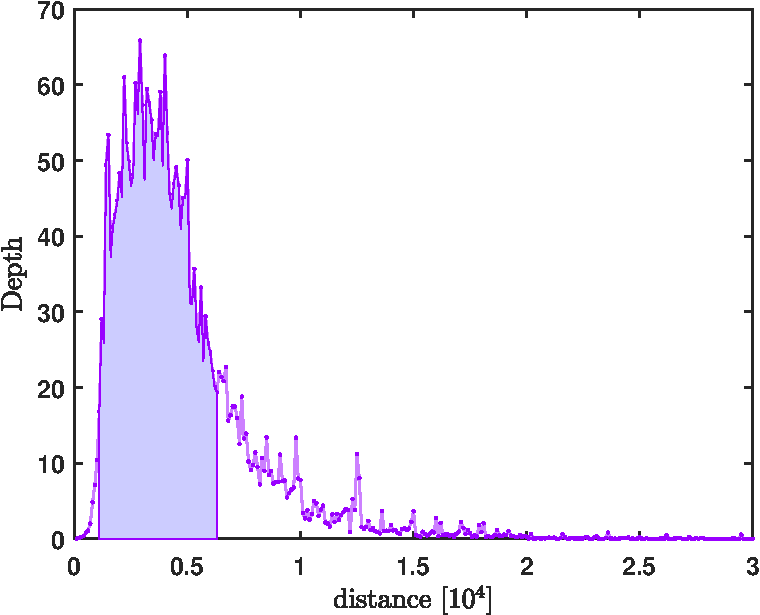
\includegraphics[width=\textwidth]{./AverageDepthProfile/TSLA/average_depth_profile.pdf}
		\caption{\ac{tsla}}
        \label{figure:average_depth:tsla}
	\end{subfigure}
	
	%--------------------------------------------------------------------------------------	
	% Caption
	%--------------------------------------------------------------------------------------
	\caption{Average depth profile of \ac{amzn}, \ac{nflx} and \ac{tsla} for the trading day 
	$4^\textrm{th}$ January $2016$. The solid blue area below the graph is bounded by the $1$\% and $80$\% 
	quantiles of the distribution. Most of the limit orders are placed near the spread. The depth of limit orders far away from the spread decays as a power law function of the distance from the best prices.}
	\label{figure:averaged_depth_profile}
	
\end{figure}
%
%-----------------------------------------------------------------------------------------
% Calibrated Model parameters 
%-----------------------------------------------------------------------------------------
%
\subsection{\ac{sfgk} parameters}

Calibrating the \ac{sfgk} using the in-sample-data by  following Sec.~\ref{section:methods:calibration} yields the model parameters that are listed in the fifth till ninth column of Table~\ref{table:calibrated_model_parameters}. The rates $\alpha$, $\mu$ and $\delta$ show a strong dependence on the trading day supporting the notion that stock markets are highly triggered by external information.

\begin{table}    
    \begin{tabular*}{\textwidth}{l|l| @{\extracolsep{\fill}} cc|ccccc}
    	\hline    	
		{\bf Stock} & {\bf Trading day} & $q_\textrm{l}$ & $q_\textrm{u}$ & $\alpha$  &  $\mu$ & $\delta$ & $\sigma$ & $\pi$\\
    	\hline
    	\ac{amzn} & 2016-01-04 & $1900$ & $10500$ & $0.0311$ & $0.557$ & $0.107$ & $72.83$ & $100$ \\
    	 		  & 2016-01-15 & $2500$ & $13100$ & $0.0249$ & $0.450$ & $0.095$ & $74.23$ & $100$ \\
    	 		  & 2016-01-29 &  $900$ & $11000$ & $0.0276$ & $0.972$ & $0.103$ & $82.29$ & $100$ \\
		\hline
		\ac{tsla} & 2016-01-04 & $1000$ &  $6400$ & $0.0320$ & $0.467$ & $0.056$ & $86.91$ & $100$ \\
    	 		  & 2016-01-15 &  $900$ &  $8300$ & $0.0286$ & $0.317$ & $0.080$ & $86.66$ & $100$ \\
    	 		  & 2016-01-29 & $1200$ &  $7000$ & $0.0161$ & $0.150$ & $0.038$ & $89.25$ & $100$ \\
		\hline
		\ac{nflx} & 2016-01-04 &  $200$ &  $2000$ & $0.3245$ & $0.767$ & $0.174$ &  $99.64$ & $100$ \\
    	 		  & 2016-01-15 &  $400$ &  $3200$ & $0.1954$ & $0.720$ & $0.156$ & $100.94$ & $100$ \\
    	 		  & 2016-01-29 &  $200$ &  $1600$ & $0.3972$ & $0.768$ & $0.128$ & $104.34$ & $100$ \\
		\hline

    \end{tabular*}
    \caption{Calibrated parameters of the \ac{sfgk} for the stocks \ac{amzn}, \ac{tsla} and \ac{nflx}.}
    \label{table:calibrated_model_parameters}
\end{table}

%-----------------------------------------------------------------------------------------
% Calibration
%----------------------------------------------------------------------------------------

\section{Simulation}
\label{section:result:simulation}

We run the calibrated \ac{sfgk} $10$ times for a length of $10^4\,$seconds for each stock and trading day using different random seeds. From the time trajectory of limit order depth profiles we determine the implied price time series (see Sec.~\ref{section:methods:price}).

Fig.~\ref{figure:result:price_evolution} depicts the $10$ different paths of price time series for \ac{amzn}, \ac{nflx} and \ac{tsla} for the trading day $4^\textrm{th}$ January $2016$. Each path is represented by a differently coloured solid line. Note that all paths for a particular stock start at the same initial price point, as they were computed from the same calibrated model. The picture reveals that on the presented time scale the price path resemble a diffusive motion. 

%--------------------------------------------------------------------------------------
% Price paths
%--------------------------------------------------------------------------------------

\begin{figure}[H]	

	\centering	
	
	%--------------------------------------------------------------------------------------	
	% Price evolution: Amazon
	%--------------------------------------------------------------------------------------
	\begin{subfigure}[b]{0.5\textwidth}
    	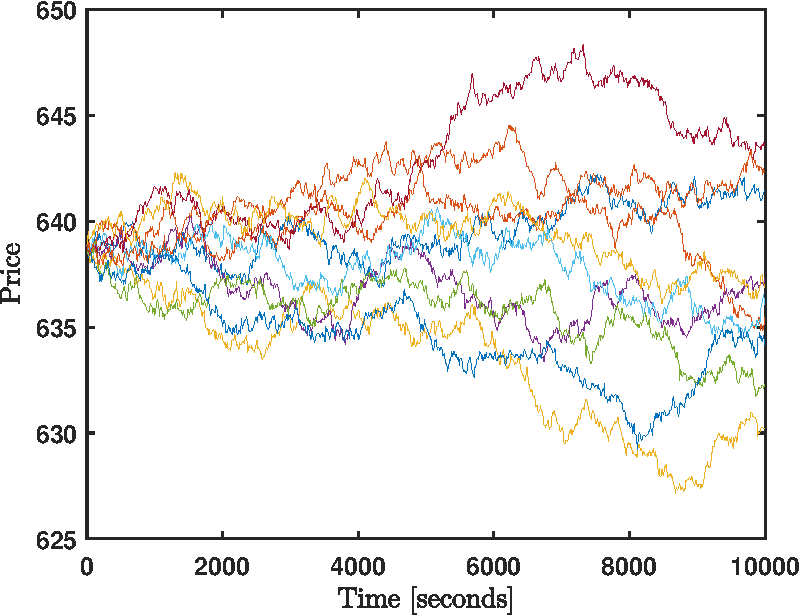
\includegraphics[width=\textwidth]{./SignaturePlot/AMZN/20160104/simulated_paths.pdf}
		\caption{\ac{amzn}}
        \label{figure:result:price_evolution:amzn}        
	\end{subfigure}	
	
	%--------------------------------------------------------------------------------------	
	% Price evolution: Netflix
	%--------------------------------------------------------------------------------------	
	\begin{subfigure}[b]{0.5\textwidth}
    	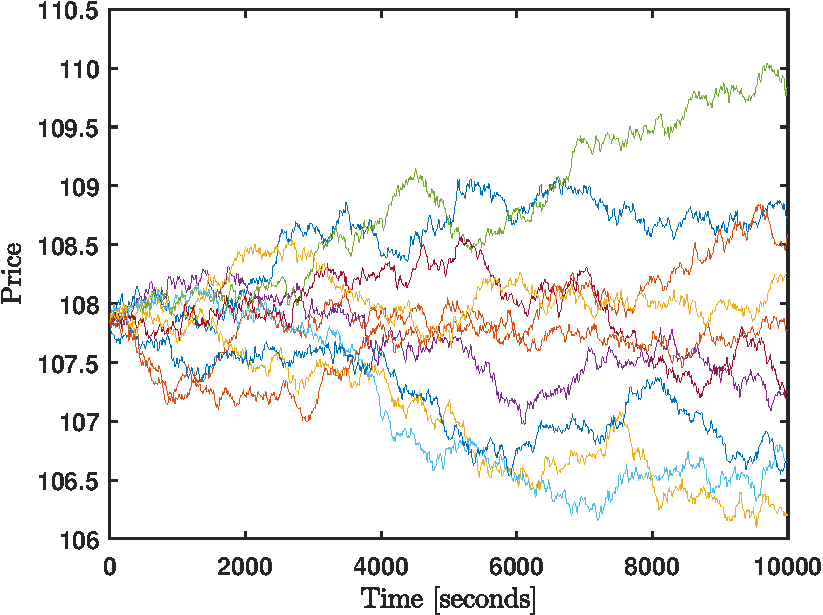
\includegraphics[width=\textwidth]{./SignaturePlot/NFLX/20160104/simulated_paths.pdf}
		\caption{\ac{nflx}}
        \label{figure:result:price_evolution:nflx}
	\end{subfigure}	
	
	%--------------------------------------------------------------------------------------	
	% Price evolution: Tesla
	%--------------------------------------------------------------------------------------
	\begin{subfigure}[b]{0.5\textwidth}
    	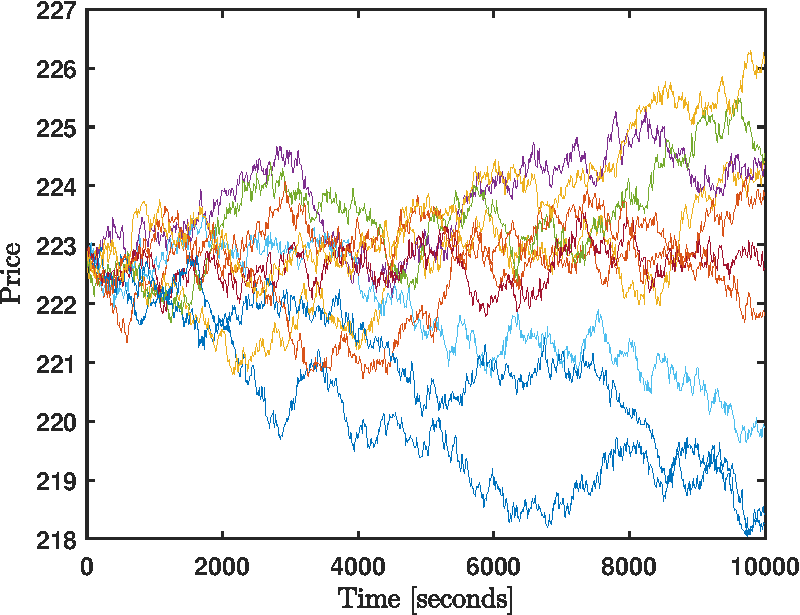
\includegraphics[width=\textwidth]{./SignaturePlot/TSLA/20160104/simulated_paths.pdf}
		\caption{\ac{tsla}}
        \label{figure:result:price_evolution:tsla}
	\end{subfigure}	

	\caption{Set of price $10$ time series for a simulation period of $10^4\,$seconds for 
	the stocks \ac{amzn}, \ac{nflx} and \ac{tsla}. The price time series was computed from 
	the \ac{sfgk} calibrated to the in-sample trading data of the respective stock for the 
	trading day $4^\textrm{th}$ January $2016$.}
	 \label{figure:result:price_evolution}
\end{figure}

%--------------------------------------------------------------------------------------
% Is price process diffusive?
%--------------------------------------------------------------------------------------

\noindent \citeauthor{Anderson:2000:GreatRealisations}~\citep{Anderson:2000:GreatRealisations}, however, argue that for smaller time scales the assumption of diffusive prices is not tolerable anymore as market micro-structure effects emerge. Market micro-structure effects can be observed by zooming into the simulated price time series as illustrated in Fig.~\ref{figure:result:micro_price_evolution:tsla}. We observe
that for a time-scale in the order of seconds the price process resembles more a step-wise
function then a random walk. The discrete nature of the simulated price evolution stems from the
fact that the order flow in the \ac{sfgk} is modelled by Poisson processes.

%--------------------------------------------------------------------------------------
% Zoomed Price paths
%--------------------------------------------------------------------------------------

\begin{figure} [H]
	\centering
	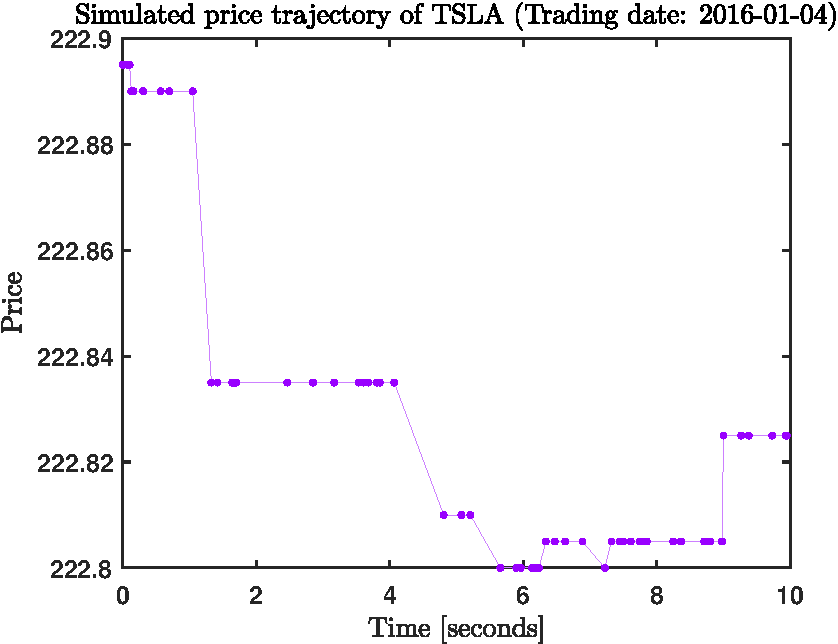
\includegraphics[width=0.8\textwidth]
	{./SignaturePlot/TSLA/20160104/price_simulated_micro_structure.pdf}
	\caption{Zooming on a smaller time scale of a price path of \ac{tsla} for trading day 
	$4^\textrm{th}$ January $2016$ reveals the discrete nature of the price process.}
	\label{figure:result:micro_price_evolution:tsla}	
\end{figure}	

%--------------------------------------------------------------------------------------
% Log price return distribution
%-------------------------------------------------------------------------------------

Fig.~\ref{figure:result:log_return} compares the distribution of log-returns from the model-implied and the empirical prices. For the latter we consider the distribution from the in-sample as well as the out-of-sample data. For \ac{tsla} we observe that the log-return distribution of the model-implied resembles the empirical distribution for the out-of-sample. This clearly demonstrates that the prices generated by the \ac{sfgk} for this particular case predict the statistical properties of  the out-of-sample prices. By contrast the model-implied log-return distribution for \ac{amzn} and \ac{nflx} does not capture the features of the empirical out-of-sample distribution, giving evidence that the \ac{sfgk} failed to predict the statistical properties.

%--------------------------------------------------------------------------------------
% Figure Log price return distribution
%-------------------------------------------------------------------------------------

\begin{figure}[H]	

	\centering	
	%--------------------------------------------------------------------------------------	
	% Log return distribution: Amazon
	%--------------------------------------------------------------------------------------
    \begin{subfigure}[b]{0.5\textwidth}
        \centering
        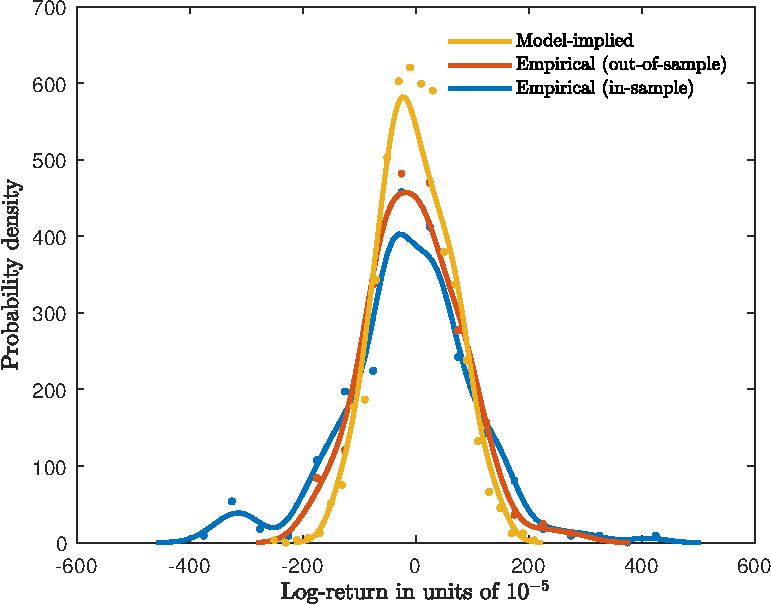
\includegraphics[width=\textwidth]{./SignaturePlot/AMZN/20160104/log_return_distribution.pdf}
        \caption{\ac{amzn}, 2016-01-04}
        \label{figure:results:log_distribution:amzn:20160104}
    \end{subfigure}
    \vfill
	%--------------------------------------------------------------------------------------	
	% Log return distribution: Netflix
	%--------------------------------------------------------------------------------------	    
    \begin{subfigure}[b]{0.5\textwidth}
        \centering
        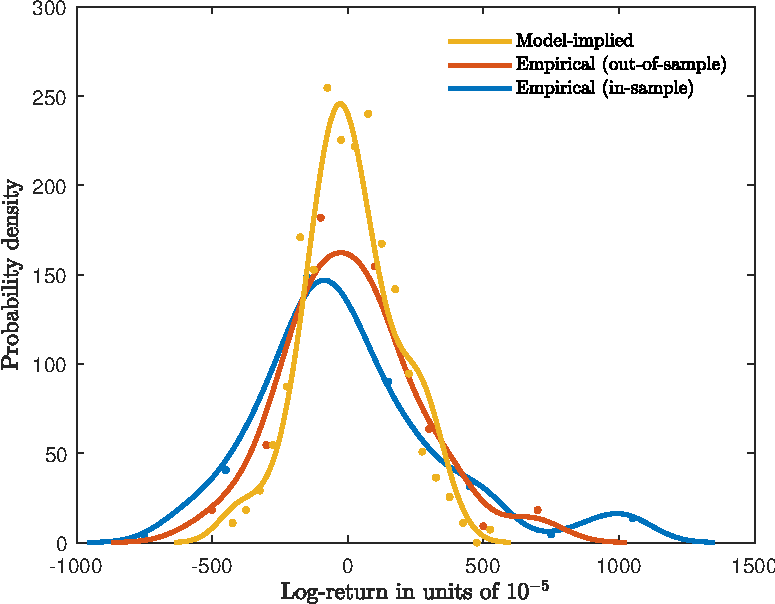
\includegraphics[width=\textwidth]{./SignaturePlot/NFLX/20160115/log_return_distribution.pdf}
        \caption{\ac{nflx}, 2016-01-15}
        \label{figure:results:log_distribution:nflx:20160104}
    \end{subfigure}
    \vfill
    %--------------------------------------------------------------------------------------	
	% Log return distribution: Tesla
	%--------------------------------------------------------------------------------------
    \begin{subfigure}[b]{0.5\textwidth}
        \centering
        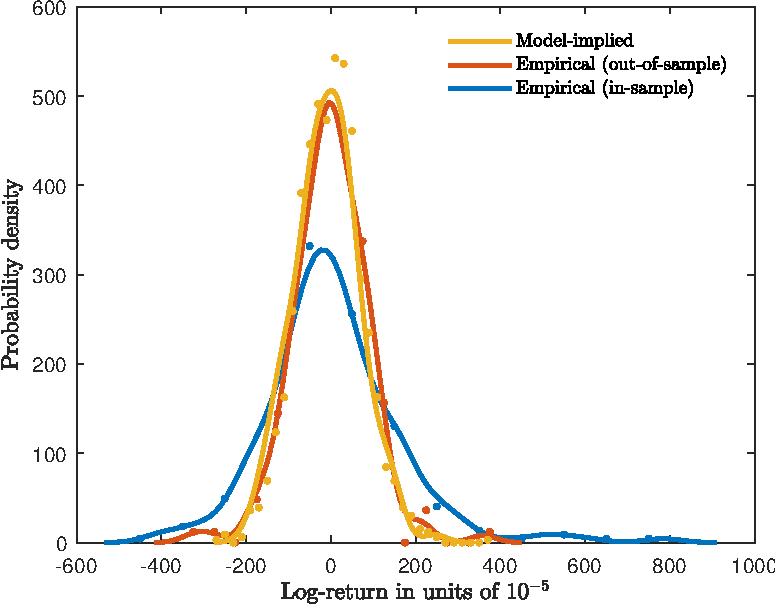
\includegraphics[width=\textwidth]{./SignaturePlot/TSLA/20160129/log_return_distribution.pdf}
        \caption{\ac{tsla}, 2016-01-29}
        \label{figure:results:log_distribution:tsla:20160104}
    \end{subfigure}

	\caption{Log-return distributions of the simulated prices of 
	the stocks \ac{amzn}, \ac{nflx} and \ac{tsla} for the 
	trading day $4^\textrm{th}$ January $2016$.}
	 \label{figure:result:log_return}
\end{figure}

%========================================================================================
%
% Realized Volatility
% 
%========================================================================================

\section{Realized Volatility}
\label{section:result:realizedvol}

In this section we begin with turning our attention to the volatility signatures that we computed from the simulated price trajectories and finally investigate to what extend the model-implied realized volatility produced by the \ac{sfgk} can forecast the empirical value extracted from out-of-sample trading data.

\subsection{Signature Plots}
\label{section:signature_plot_discussion}
To provide a concrete example, we start by analysing the model-implied realized volatility signature of \ac{tsla} for the trading day $4^\textrm{th}$ January $2016$. 
%
%-----------------------------------------------------------------------------------------
% Volatility Signature Plot: TSL, 04.01.2016
%-----------------------------------------------------------------------------------------
%
\begin{figure}[H]
	\centering
	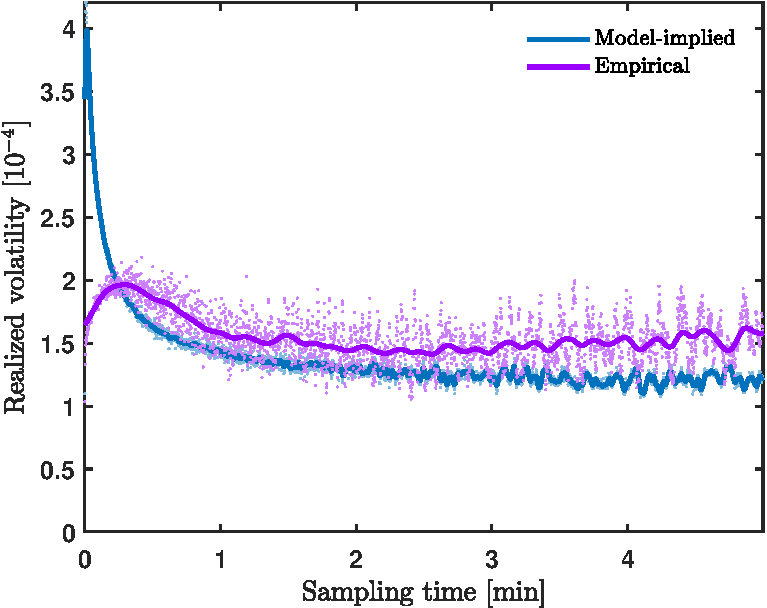
\includegraphics[width=0.8\textwidth]
	{./SignaturePlot/TSLA/20160104/signature_plot_predicted_vs_measured.pdf}
	\caption{Model-implied (turquoise) versus the empirical (purple) realized volatility signature of \ac{tsla} for trading day $4^\textrm{th}$ January $2016$.}
	\label{figure:results:signature_plot:tsla:20160104:detail}
\end{figure}
%
% Short description of the figure
%
Fig.~\ref{figure:results:signature_plot:tsla:20160104:detail} depicts the model-implied and empirical realized volatility depending on the sampling frequency $\delta t$ of \ac{tsla} for the trading day $4^\textrm{th}$ January $20$, denoted by turquoise and purple solid line, respectively. Note that the solid lines are guides to the eye and were determined by averaging the computed values (dots) in order to reduce the noise. In the following we will refer to realized volatility versus sampling frequency plots to as {\it volatility signature}~\citep{Anderson:2000:GreatRealisations}.
% 
% Start the observation
%
We observe that both the model-implied as well as the empirical realized volatility significantly deviates for $\delta t<1\,\textrm{min}$ from its plateau value that we observe for $\delta t>1\,\textrm{min}$. Assuming that the price process is diffusive we would expect a convergence of the realized volatility for decreasing sampling frequency as explained in Sec.~\ref{section:realized_vol}. \citeauthor{Anderson:2000:GreatRealisations}~\citep{Anderson:2000:GreatRealisations} argues that for smaller time scales the assumption of diffusive prices is not tolerable any more as market micro-structure effects emerge. For sampling frequencies larger than $1\,$min the realized volatility stabilises and reaches a plateau. By averaging the values for $\delta t \ge 1\,$min we obtain, for the empirical and model-implied realized volatility, $(1.48\pm 0.26)\cdot 10^{-4}$ and $(1.27\pm 0.18)\cdot 10^{-4}$, respectively. Hence, the model-implied value is forecasting the empirical value within the error bounds. Its noteworthy that the empirical points are initially below, and subsequently above, the model-implied values. Furthermore, for very small sampling frequencies the model-implied volatility is significantly larger then the empirical volatility.

% [TODO] Seperate section?
% Lets check all the othere
%
Fig.~\ref{figure:results:signature_plots} shows the volatility signature of the model-implied (turquoise solid line) and the empirical realized volatility (purple solid line) for \ac{amzn}, \ac{nflx} and \ac{tsla} for the trading days $4^\textrm{th}$, $15^\textrm{th}$ and $29^\textrm{th}$ January $2016$. We observe the follow points: 

\begin{itemize}

	\item The shape of the empirical and model-implied volatility signature deviate in the majority of cases, indicating that \ac{sfgk} captures less features of the limit order book dynamics.
	
	\item It may be conjectured that the shape of the model-implied volatility signature can be described in terms of an exponential decay of the form $\textrm{RV}(\delta t) = a\,e^{-b\,\delta t}+c$.
	
	\item The model-implied realized volatility values have the correct order of magnitude when compared to the empirical values.
	
	\item For the majority of cases the model-implied and the empirical volatility signatures deviate from each other. Apart from the volatility signature of \ac{amzn} for the trading day $29^\textrm{th}$ January $2016$, the model-implied realized volatility underestimated the empirical realized volatility for sampling frequencies $\delta t  \ge 1\,$ minute.
		
\end{itemize}

%-----------------------------------------------------------------------------------------
% Volatility Signature Plot: for all
%-----------------------------------------------------------------------------------------

\begin{figure}[H]
    \centering
    
    %----------------------------------------------------------------------------
	% AMZN    
    %----------------------------------------------------------------------------

    \begin{subfigure}[b]{0.3\textwidth}
        \centering
        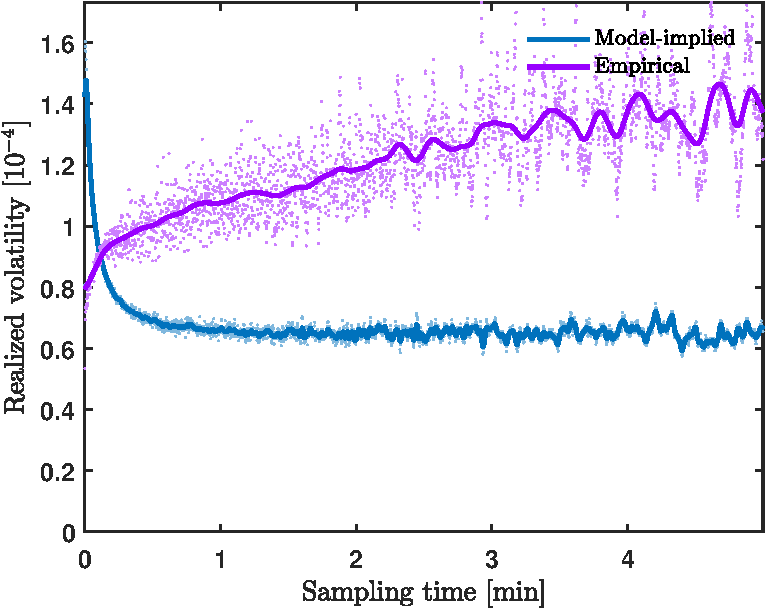
\includegraphics[width=\textwidth]{./SignaturePlot/AMZN/20160104/signature_plot_predicted_vs_measured.pdf}
        \caption{\ac{amzn}, 2016-01-04}
        \label{figure:results:signature_plot:amzn:20160104}
    \end{subfigure}
    \hfill
    \begin{subfigure}[b]{0.3\textwidth}
        \centering
        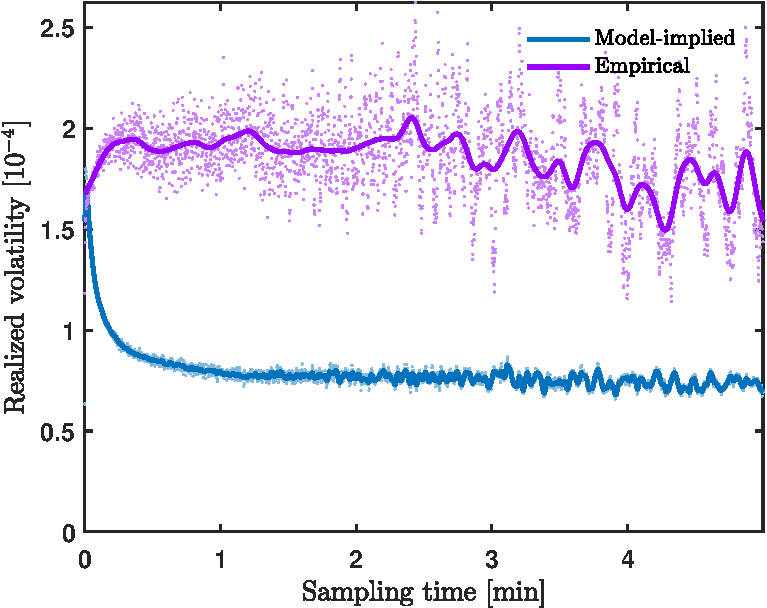
\includegraphics[width=\textwidth]{./SignaturePlot/AMZN/20160115/signature_plot_predicted_vs_measured.pdf}
        \caption{\ac{amzn}, 2016-01-15}
        \label{figure:results:signature_plot:amzn:20160115}
    \end{subfigure}
    \hfill
    \begin{subfigure}[b]{0.3\textwidth}
        \centering
        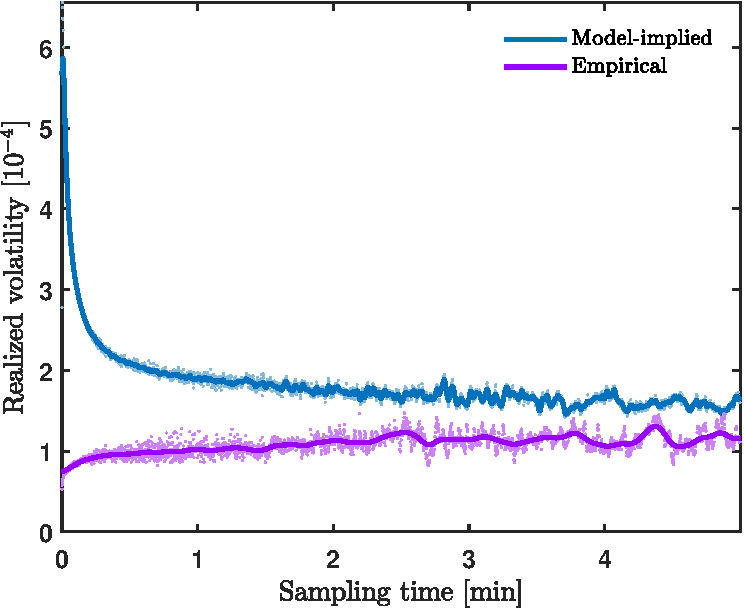
\includegraphics[width=\textwidth]{./SignaturePlot/AMZN/20160129/signature_plot_predicted_vs_measured.pdf}
        \caption{\ac{amzn}, 2016-01-29}
        \label{figure:results:signature_plot:amzn:20160129}
    \end{subfigure}

    \vfill
    
    %----------------------------------------------------------------------------
	% NFLX    
    %----------------------------------------------------------------------------

    \begin{subfigure}[b]{0.3\textwidth}
        \centering
        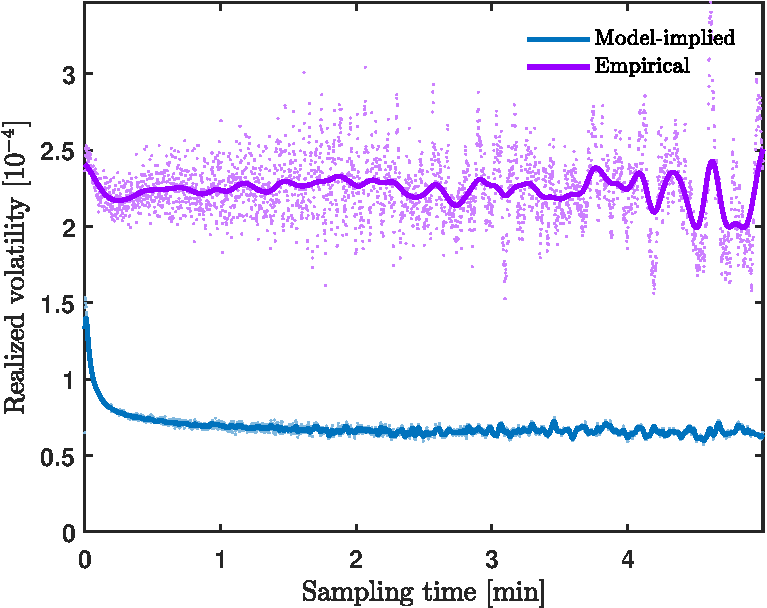
\includegraphics[width=\textwidth]{./SignaturePlot/NFLX/20160104/signature_plot_predicted_vs_measured.pdf}
        \caption{\ac{nflx}, 2016-01-04}
        \label{figure:results:signature_plot:nflx:20160104}
    \end{subfigure}
    \hfill
    \begin{subfigure}[b]{0.3\textwidth}
        \centering
        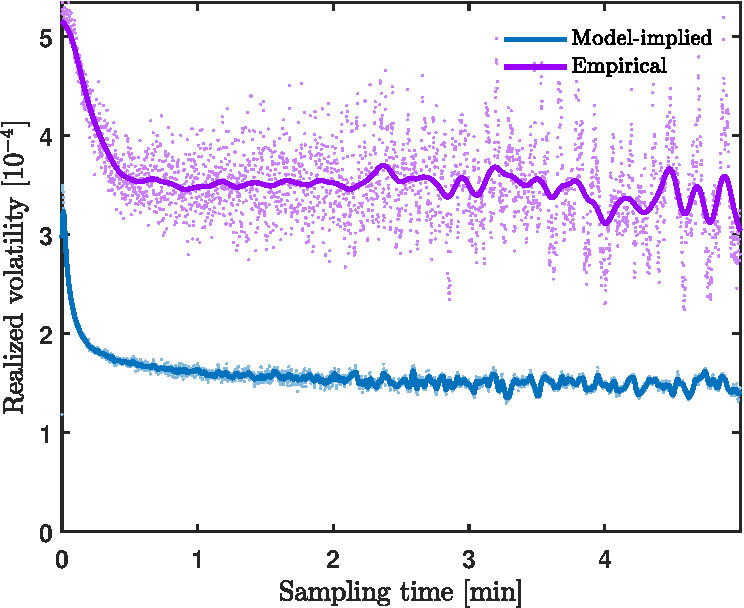
\includegraphics[width=\textwidth]{./SignaturePlot/NFLX/20160115/signature_plot_predicted_vs_measured.pdf}
        \caption{\ac{nflx}, 2016-01-15}
        \label{figure:results:signature_plot:nflx:20160115}
    \end{subfigure}
    \hfill
    \begin{subfigure}[b]{0.3\textwidth}
        \centering
        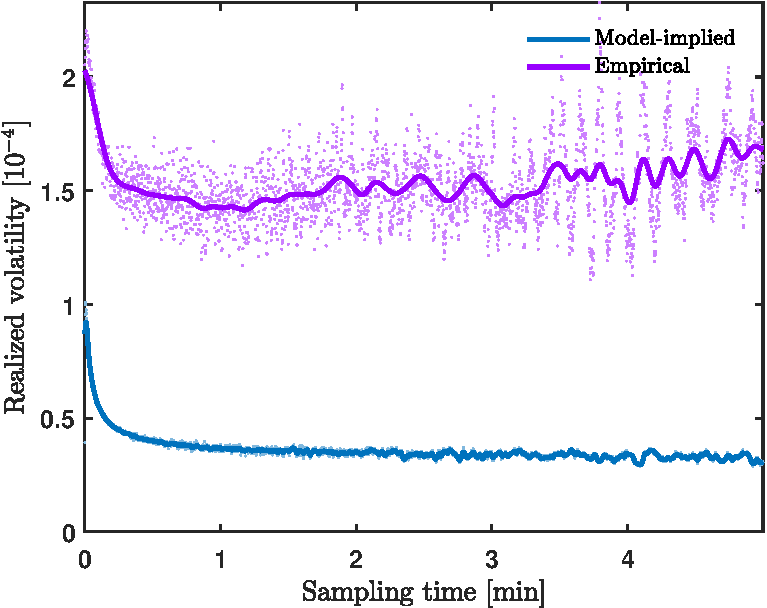
\includegraphics[width=\textwidth]{./SignaturePlot/NFLX/20160129/signature_plot_predicted_vs_measured.pdf}
        \caption{\ac{nflx}, 2016-01-29}
        \label{figure:results:signature_plot:nflx:20160129}
    \end{subfigure}
    
    \vfill
    
    %----------------------------------------------------------------------------
	% TSLA    
    %----------------------------------------------------------------------------

    \begin{subfigure}[b]{0.3\textwidth}
        \centering
        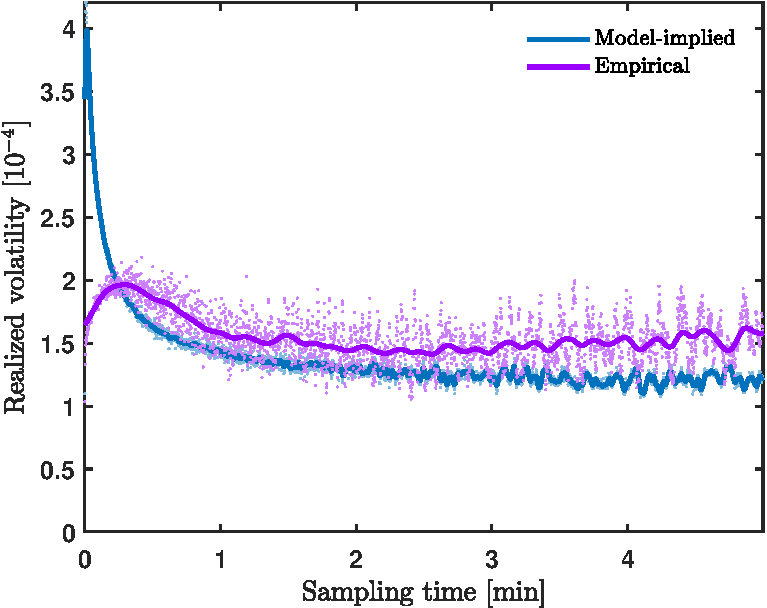
\includegraphics[width=\textwidth]{./SignaturePlot/TSLA/20160104/signature_plot_predicted_vs_measured.pdf}
        \caption{\ac{tsla}, 2016-01-04}
        \label{figure:results:signature_plot:tsla:20160104}
    \end{subfigure}
    \hfill
    \begin{subfigure}[b]{0.3\textwidth}
        \centering
        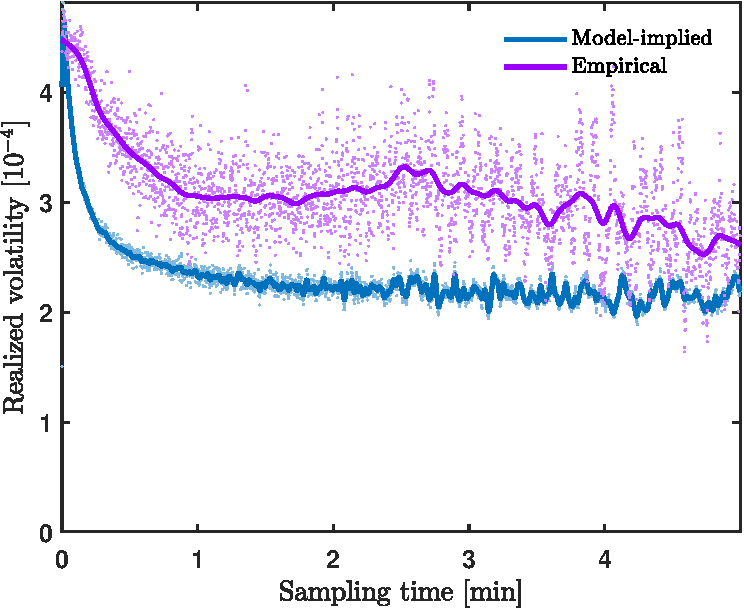
\includegraphics[width=\textwidth]{./SignaturePlot/TSLA/20160115/signature_plot_predicted_vs_measured.pdf}
        \caption{\ac{tsla}, 2016-01-15}
        \label{figure:results:signature_plot:tsla:20160115}
    \end{subfigure}
    \hfill
    \begin{subfigure}[b]{0.3\textwidth}
        \centering
        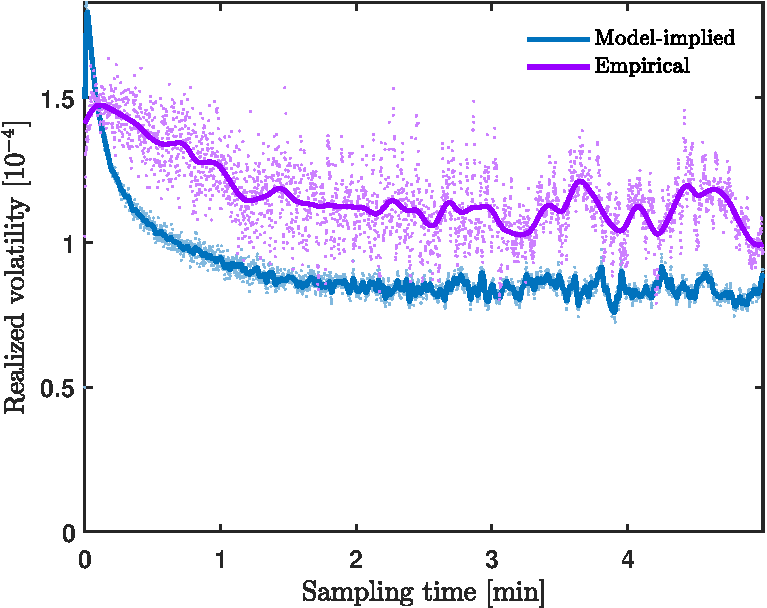
\includegraphics[width=\textwidth]{./SignaturePlot/TSLA/20160129/signature_plot_predicted_vs_measured.pdf}
        \caption{\ac{tsla}, 2016-01-29}
        \label{figure:results:signature_plot:tsla:20160129}
    \end{subfigure}
    
   	%----------------------------------------------------------------------------
	% Caption  
    %----------------------------------------------------------------------------

    \caption{Model-implied (turquoise solid line) and empirical (purple solid line) 
	realized volatility depending on the sampling frequency for \ac{amzn}, \ac{nflx} and 
	\ac{tsla} for the trading days $4^\textrm{th}$, $15^\textrm{th}$ and $29^\textrm{th}$ January $2016$.}
    \label{figure:results:signature_plots}
\end{figure}


%-----------------------------------------------------------------------------------------
% 
% LO interarival times: TSL
% TODO: Do we also need MO, CO-tau here?
%
%-----------------------------------------------------------------------------------------

%\begin{figure}[htp]		
%    \includegraphics[width=\textwidth]
%    {./InterarrivalTimeDistribution/TSLA/distribution_limit_order_interarrival_times.pdf}
%	\caption{Probability density distribution of the logarithm of \ac{lo} interarrival times for \ac{tsla}. The \ac{lo} interrarival time $\tau$ is the time span between two consecutive placements of a \ac{lo} into the \ac{lob}. Hence, $\tau$ reflects the time scale of changes of the state of the \ac{lob} and thereby the price process. Furthermore it gives a estimate of the time scale on which market micro structure effects emerges. Note that the interarrival times were computed from the \ac{lo} events of the trading data of \ac{tsla} for all trading days.}
%	\label{figure:interarrival_time:tsla}
%\end{figure}


\subsection{Forecasting performance}
% [TODO] Reformulate
Fig.~\ref{figure:results:realized_volatility_vs_trading_date} show the model-implied realized volatility determined from the volatility signatures by averaging the sampling frequency dependent realized volatilities for $\delta t \ge 1\,$min. For \ac{tsla} (Fig.~\ref{figure:results:realized_volatility_vs_trading_date:tsla}) the realized volatility is predicted correctly within the error bars. For \ac{nflx} the realized volatility is underestimated but yields the correct order of magnitude. Furthermore, we observe that the model-implied and the empirical volatility show the same dependence on the trading day, indicating that \ac{sfgk} captures the correct behaviour of increasing and decreasing volatility. By contrast, for \ac{amzn} the realized and the empirical realized volatility have solely the same order of magnitude. 

%-----------------------------------------------------------------------------------------
%
% Figure: model-implied versus empirical realized volatility
%
%-----------------------------------------------------------------------------------------

\begin{figure}[H]
	
	%----------------------------------------------------------------------------
	% Realized volatility: AMZN
	%----------------------------------------------------------------------------
	\begin{subfigure}[b]{0.3\textwidth}
        \centering
        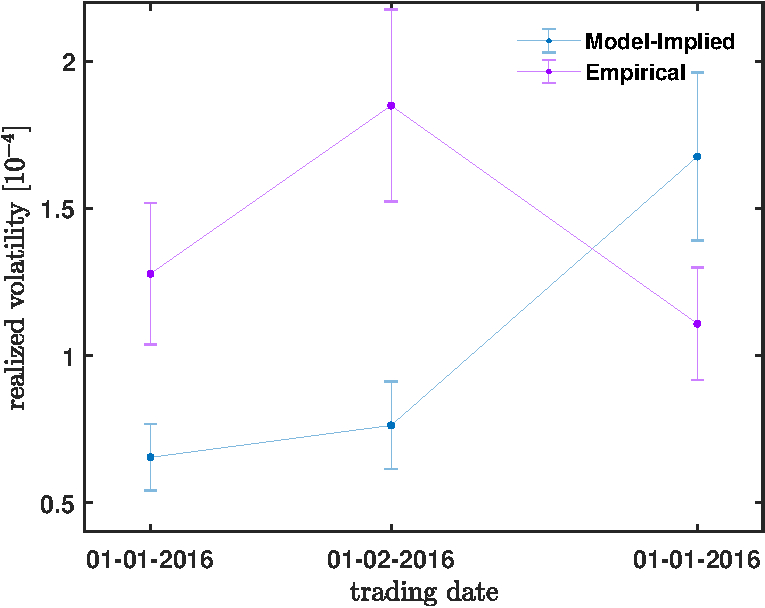
\includegraphics[width=\textwidth]{./RealizedVolatility/AMZN/realized_volatility_predicted_vs_actual.pdf}
        \caption{\ac{amzn}}
        \label{figure:results:realized_volatility_vs_trading_date:amzn}
    \end{subfigure}
    \hfill
	%----------------------------------------------------------------------------
	% Realized volatility: NFLX
	%-------------------------------------------------------------------------
	\begin{subfigure}[b]{0.3\textwidth}
        \centering
        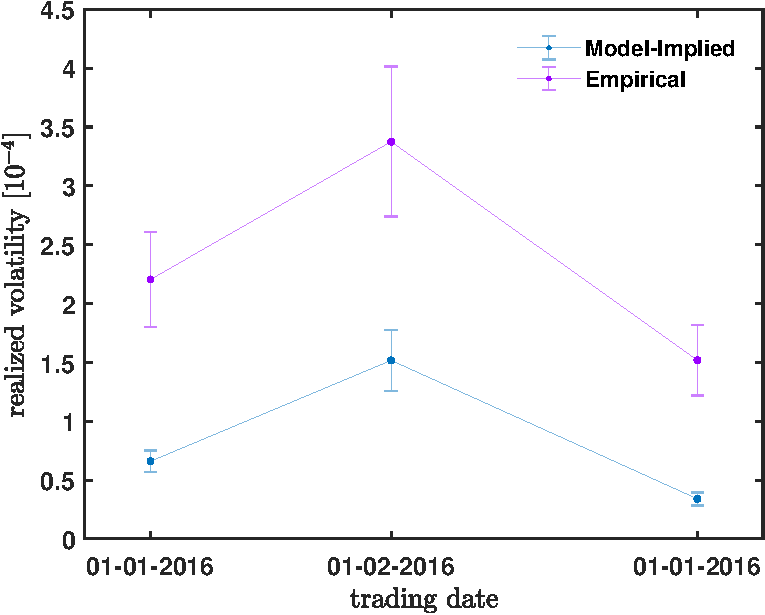
\includegraphics[width=\textwidth]{./RealizedVolatility/NFLX/realized_volatility_predicted_vs_actual.pdf}
        \caption{\ac{nflx}}
        \label{figure:results:realized_volatility_vs_trading_date:nflx}
    \end{subfigure}
    \hfill
	%----------------------------------------------------------------------------
	% Realized volatility: TSLA
	%----------------------------------------------------------------------------
	\begin{subfigure}[b]{0.3\textwidth}
        \centering
        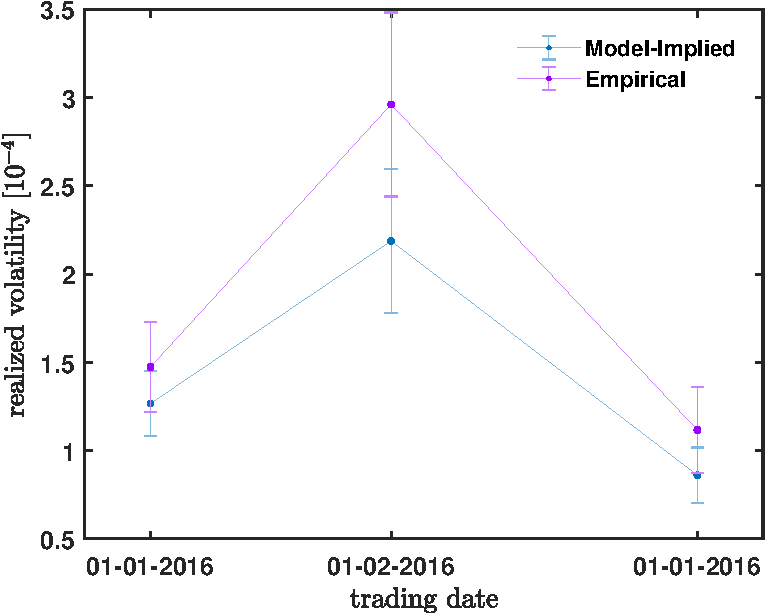
\includegraphics[width=\textwidth]{./RealizedVolatility/TSLA/realized_volatility_predicted_vs_actual.pdf}
        \caption{\ac{tsla}}
        \label{figure:results:realized_volatility_vs_trading_date:tsla}
    \end{subfigure}
	
	%----------------------------------------------------------------------------
	% Caption
	%----------------------------------------------------------------------------
	\caption{Model-implied (turquoise) versus empirical (purple) realized volatility 
	for the stocks \ac{amzn}, \ac{nflx} and \ac{tsla} for different trading days.}	
	\label{figure:results:realized_volatility_vs_trading_date}
\end{figure}

%*****************************************************************************************
%
% Summary & Conclusion 
% Notes:
% - Order arrive simulatnously, cannot be captured by a Poisson process. As possion proccess 
% assumed that order arive one after the another.  
% Check percentage of order that arrive simultaneously. For example, in the data set for the ticker GOOG % that we are analysing
% in this dissertation, 2.69% of LOs and MOs arrive simultaneously.
%*****************************************************************************************

\chapter{Summary \& Conclusion}
\label{chapter:summary_conclusions}
%----------------------------------------------------------------------------------------
% Short summary of what we have done
%----------------------------------------------------------------------------------------

In this thesis we have investigated the forecasting performance of the model-implied realized volatility using the \ac{sfgk} in conjunction with a simple realized estimator proposed by \citeauthor{Anderson:2000:GreatRealisations}~\cite{Anderson:2000:GreatRealisations}. To this end we have,  

\begin{itemize}

	\item Implemented the \ac{sfgk} by restricting it to a finite price interval.
		
	\item Calibrated the \ac{sfgk} to a set of in-sample trading data for \ac{amzn}, \ac{tsla} and \ac{nflx}.
	
	\item Run the calibrated models and generated a set of price trajectories from which we determined the predictions for the realized volatility. 
	
	\item Compared the predicted realized volatility value with the empirical realized volatility values extracted from the out-of-sample data.
\end{itemize} 

%----------------------------------------------------------------------------------------
% Main result
%----------------------------------------------------------------------------------------

The main result of this thesis can be summarized as follows: We have found that the \ac{sfgk} in  combination with a simple estimator fails to accurately predict the realized volatility. Interestingly, it capture the realized volatility on the correct order of magnitude. In a few rare cases, it even capture the realized volatility within the errorbars (see Sec.~\ref{section:signature_plot_discussion}). We have to stress here, that the \ac{sfgk} is a very simplistic model, only described by five parameters and simple Poisson processes, therefore not capturing features such as clustering or the synchronous submission of orders.  From this perspective it is striking that the realized volatility can be predicted on the correct order of magnitude, and it comes to no surprise, that it fails to correctly predict the realized volatility. 
%
%----------------------------------------------------------------------------------------
% Outlook
%----------------------------------------------------------------------------------------
\\
\\
\noindent Therefore the usage of the simplistic \ac{sfgk} zero-intelligence model should be regarded as a starting point from which we can add more complex features in order to improve its forecasting performance with respect to the realized volatility. Concluding this thesis, we mention a list of possibilities for future extension of this work:

\begin{itemize}

	\item Instead of using a simple realized volatility estimator, use more elaborated realized volatility estimators that are robust to market micro-structure noise ~\cite{Andersen:2010:volatility_measurement}.
	
	\item Investigate which feature cannot be captured by the \ac{sfgk} and focus to improve the model. For instance begin with improving the cancellation mechanism as most orders are cancelled or deleted. A good starting point might the work of 	\citeauthor{Cont:2010:model}~\cite{Cont:2010:model}.
	
	\item Using Poisson processes excludes certain features such as clustering and the synchronous placement of  orders. We propose to use other stochastic processes to model the order flow that can capture those features..	

	\item Use more complex agent based models with learning features that better capture the rich features of the limit order book dynamic.
	
\end{itemize}
 
%*****************************************************************************************
%
% Appendix
%
%*****************************************************************************************

\appendix

%-----------------------------------------------------------------------------------------
% C#-implementattion 
%-----------------------------------------------------------------------------------------

\chapter{Implementation}
\label{section:implementation}

%-----------------------------------------------------------------------------------------
% Introduction
%-----------------------------------------------------------------------------------------

In this chapter we give a short overview over the source code that was developed by the author of this thesis to analyse the predictably of the \ac{sfgk} with regards to the realized volatility. All source code is provided as supplementary material to this thesis.

%-----------------------------------------------------------------------------------------
% Simulation unsing C#
%-----------------------------------------------------------------------------------------
\section{Order flow model}
\label{section:implementation:order_flow_model}

For modelling price time series as input for the realized volatility we implemented the \ac{sfgk} using the C\# programming language. The source code can be found in the folder {\bf \texttt{C\#\_Smith\_et\_al\_Model}}.  For the sake of generalization we separated the implementation of the \ac{lob} (see Sec.~\ref{section:lob}) from the simulation of the order flow (see Sec.~\ref{section:order_flow_model:algorithm}). 

\subsection{Limit order book}
The relevant source code is defined in the class {\bf LimitOrderBook}. For performance reasons, we use a sorted dictionary for the sell as well the buy side, 
%
\begin{lstlisting}
public class LimitOrderBook : ILimitOrderBook
{
  public double Time { get; set; }
  private SortedDictionary<int, int> DepthSellSide { get; }
  private SortedDictionary<int, int> DepthBuySide { get; }
  ...
}
\end{lstlisting}
%
The dictionaries {\bf DepthBuySide} and {\bf DepthSellSide} are an implementation of both mappings $p \rightarrow n^b(t, p)$ and $p \rightarrow n^a(t, p)$ (see Eq.~\ref{equation:depth}), respectively. Methods for submitting or cancelling order in the class {\bf LimitOrderBook} changing the the bid and ask-side depth profiles accordingly.

\subsection{Order flow} 

The class {\bf SmithFarmerModel} implements the order flow logic as described in Sec.~\ref{section:order_flow_model:algorithm}). As mentioned in Sec.~\ref{section:order_flow_model:theory} we place \acp{lo} on a finite price interval as practical simplification of the infinite interval as originally proposed by \citeauthor{Smith:2003:StatisticalModel}~\cite{Smith:2003:StatisticalModel}. The order flow interacts with \ac{lob} by means of a general interface such that the underlying \ac{lob} implementation can be replaced. Furthermore the Poisson process generating the order events can readily be replaced to extend the model to more sophisticated processes. 

\subsection{Calibration} 

In order to calibrate the model parameter in Table~\ref{table:model_parameter}, we implemented the calibration described in Sec.~\ref{section:methods:calibration} with the class {\bf SmithFarmerModelCalibration}. 

% TODO: Notes on performance
% What is the best structure for limit order book?
% => Simple array based implementation?
% => However, note that it will be less optimal when price levels are sparse and we care about every price level	
%	=> Linked-list ordered by price levels will be very efficient	

%-----------------------------------------------------------------------------------------
% Analysis using MATALB
%-----------------------------------------------------------------------------------------

\section{Preprocessing \& analysis scripts} 
\label{section:implementation:scripts}

Using the scripting language MATLAB we developed tools to pre-process the simulated price time series, and to analyse their statistical properties. The scripts can be found in the folder {\bf \texttt{Matlab\_Scripts}}. In the following we give a short overview over the scripts that were used to generate the results in Chapter~\ref{chapter:results}.

\subsection{Pre-processing} 

Price time series simulated with the \ac{sfgk} are irregularly spaced, as order events occurs randomly following a Poisson process with various rates. For the further analysis, particularly for computing the realized volatility Eq.~\ref{equation:realized_volatility_estimator}, we need, however, regularly spaced series. For this purpose we pre-process all price time series with the script {\bf \texttt{step\_1\_preprocess\_simulation}} by re-sampling the price series onto a regular grid with spacing $\Delta t=10\,$ms, sufficiently small to compute the realized volatility with a sampling frequency in the time order of minutes. 

\subsection{Control calibration} 

In order to control the calibrated parameters of the  \ac{sfgk} we developed the script {\bf \texttt{step\_2\_analyze\_calibration}}. It merely allows to plot the calibrated model parameters (see Table~\ref{table:model_parameter}) for each stock versus the trading day.

\subsection{Realized volatility of price time series} 

The realized volatility Eq.~\ref{equation:realized_volatility_estimator} is calculated with the function {\bf \texttt{realized\_volatility}} from the pre-processed price time series. In addition the function also returns asymptotic error approximation  towards the quadratic variation  proposed by \citeauthor{BarndorffNielsen:2002:EcoAnalysis}~\cite{BarndorffNielsen:2002:EcoAnalysis}. Finally, to calculate the realized volatility versus the multiples $k$ of the smallest sampling frequency $\Delta t=10\,$ms ranging from $1$ to  $30000$ in steps of $10$ for all stocks and trading days, we employ the script {\bf \texttt{step\_3\_analyze\_simulation}} on the pre-processed time series. As for each stock and trading day we have simulated $10$ random price paths with the \ac{sfgk}, we additional average the signature plot over those paths.

\subsection{Log returns of price time series} 

For analysing the realized volatility plots it is helpful to also investigate how the simulated price time series predict the statistical behaviour of the out-of-sample data. To this end, we use the script {\bf \texttt{step\_4\_analyse\_log\_returns}} to determine the distribution log-return Eq.~\ref{equation:log_return} of the in-sample, out-of-sample and simulated price time series. For ~\ac{tsla} and \ac{amzn} we use a time interval length of $1$ and for \ac{nflx} $3$ minutes.

\subsection{Interarrival times} 

In order to investigate how well the \ac{sfgk} simulates the time behaviour of the order flows we use the script{\bf \texttt{step\_5\_analyse\_interarival\_time}} to compute the distribution of interarrival times of \ac{lo}, \ac{mo} and \ac{co} events for all stocks and trading days.

%*****************************************************************************************
%
% References
%
%*****************************************************************************************

%next line adds the Bibliography to the contents page
\addcontentsline{toc}{chapter}{Bibliography}
%uncomment next line to change bibliography name to references
%\renewcommand{\bibname}{References}
\bibliographystyle{plainnat}
\bibliography{references_papers}        %use a bibtex bibliography file references.bib
%\bibliographystyle{plain}  %use the plain bibliography style

%*****************************************************************************************
%
% Acronyms
%
%*****************************************************************************************

\begin{acronym}[ECU]
	\acro{nasdaq}[NASDAQ]{\href{https://www.nasdaq.com/}
	{National Association of Securities Dealers Automated Quotations}}
	\acro{sfgk}[Smith {\it et al} model]{Smith-Farmer-Gillemot-Krishnamurthy Model~\cite{Farmer:2005:Model}}
	\acro{amzn}[AMZN]{\href{https://www.nasdaq.com/symbol/amzn/real-time}{Amazon.com, Inc Stock}}
	\acro{nflx}[NFLX]{\href{https://www.nasdaq.com/symbol/nflx/real-time}{Netflix, Inc. Stock}}
	\acro{tsla}[TSLA]{\href{https://www.nasdaq.com/symbol/tsla/real-time}{Tesla, Inc. Stock}}
	\acro{lo}[LO]{Limit order}
	\acro{mo}[MO]{Market order}
	\acro{co}[CO]{Cancel order}
	\acro{lob}[LOB]{Limit order book}
	\acro{lobster}[LOBSTER]{\href{https://lobsterdata.com/}{Limit Order Book – The Efficient Reconstructor}}
\end{acronym}

\end{document}
